\documentclass[twoside]{book}

% Packages required by doxygen
\usepackage{calc}
\usepackage{doxygen}
\usepackage{graphicx}
\usepackage[utf8]{inputenc}
\usepackage{makeidx}
\usepackage{multicol}
\usepackage{multirow}
\usepackage{textcomp}
\usepackage[table]{xcolor}

% NLS support packages
%\usepackage[T2A]{fontenc}
\usepackage[hungarian]{babel}

% Font selection
\usepackage[T1]{fontenc}
\usepackage{mathptmx}
\usepackage[scaled=.90]{helvet}
\usepackage{courier}
\usepackage{amssymb}
\usepackage{sectsty}
\renewcommand{\familydefault}{\sfdefault}
\allsectionsfont{%
  \fontseries{bc}\selectfont%
  \color{darkgray}%
}
\renewcommand{\DoxyLabelFont}{%
  \fontseries{bc}\selectfont%
  \color{darkgray}%
}

% Page & text layout
\usepackage{geometry}
\geometry{%
  a4paper,%
  top=2.5cm,%
  bottom=2.5cm,%
  left=2.5cm,%
  right=2.5cm%
}
\tolerance=750
\hfuzz=15pt
\hbadness=750
\setlength{\emergencystretch}{15pt}
\setlength{\parindent}{0cm}
\setlength{\parskip}{0.2cm}
\makeatletter
\renewcommand{\paragraph}{%
  \@startsection{paragraph}{4}{0ex}{-1.0ex}{1.0ex}{%
    \normalfont\normalsize\bfseries\SS@parafont%
  }%
}
\renewcommand{\subparagraph}{%
  \@startsection{subparagraph}{5}{0ex}{-1.0ex}{1.0ex}{%
    \normalfont\normalsize\bfseries\SS@subparafont%
  }%
}
\makeatother

% Headers & footers
\usepackage{fancyhdr}
\pagestyle{fancyplain}
\fancyhead[LE]{\fancyplain{}{\bfseries\thepage}}
\fancyhead[CE]{\fancyplain{}{}}
\fancyhead[RE]{\fancyplain{}{\bfseries\leftmark}}
\fancyhead[LO]{\fancyplain{}{\bfseries\rightmark}}
\fancyhead[CO]{\fancyplain{}{}}
\fancyhead[RO]{\fancyplain{}{\bfseries\thepage}}
\fancyfoot[LE]{\fancyplain{}{}}
\fancyfoot[CE]{\fancyplain{}{}}
\fancyfoot[RE]{\fancyplain{}{\bfseries\scriptsize Projekt: altimeter Készült: Sat Nov 29 2014 15:18:14 Készítette:  Doxygen }}
\fancyfoot[LO]{\fancyplain{}{\bfseries\scriptsize Projekt: altimeter Készült: Sat Nov 29 2014 15:18:14 Készítette:  Doxygen }}
\fancyfoot[CO]{\fancyplain{}{}}
\fancyfoot[RO]{\fancyplain{}{}}
\renewcommand{\footrulewidth}{0.4pt}
\renewcommand{\chaptermark}[1]{%
  \markboth{#1}{}%
}
\renewcommand{\sectionmark}[1]{%
  \markright{\thesection\ #1}%
}

% Indices & bibliography
\usepackage{natbib}
\usepackage[titles]{tocloft}
\setcounter{tocdepth}{3}
\setcounter{secnumdepth}{5}
\makeindex

% Custom commands
\newcommand{\clearemptydoublepage}{%
  \newpage{\pagestyle{empty}\cleardoublepage}%
}


%===== C O N T E N T S =====

\begin{document}

% Titlepage & ToC
\pagenumbering{roman}
\begin{titlepage}
\vspace*{7cm}
\begin{center}%
{\Large altimeter }\\
\vspace*{1cm}
{\large Készítette Doxygen 1.8.4}\\
\vspace*{0.5cm}
{\small Sat Nov 29 2014 15:18:14}\\
\end{center}
\end{titlepage}
\clearemptydoublepage
\tableofcontents
\clearemptydoublepage
\pagenumbering{arabic}

%--- Begin generated contents ---
\chapter{Adatszerkezet-\/mutató}
\section{Adatszerkezetek}
Az összes adatszerkezet listája rövid leírásokkal\-:\begin{DoxyCompactList}
\item\contentsline{section}{{\bf log\-\_\-rec\-\_\-ext\-\_\-s} }{\pageref{structlog__rec__ext__s}}{}
\end{DoxyCompactList}

\chapter{Fájlmutató}
\section{Fájllista}
Az összes fájl listája rövid leírásokkal\-:\begin{DoxyCompactList}
\item\contentsline{section}{src/{\bf Descriptors.\-c} }{\pageref{_descriptors_8c}}{}
\item\contentsline{section}{src/{\bf eeprom.\-c} }{\pageref{eeprom_8c}}{}
\item\contentsline{section}{src/{\bf H\-P03.\-c} }{\pageref{_h_p03_8c}}{}
\item\contentsline{section}{src/{\bf itoa.\-c} }{\pageref{itoa_8c}}{}
\item\contentsline{section}{src/{\bf Kalman.\-c} }{\pageref{_kalman_8c}}{}
\item\contentsline{section}{src/{\bf L\-C\-D.\-c} }{\pageref{_l_c_d_8c}}{}
\item\contentsline{section}{src/{\bf logger.\-c} }{\pageref{logger_8c}}{}
\item\contentsline{section}{src/{\bf main.\-c} }{\pageref{main_8c}}{}
\item\contentsline{section}{src/{\bf mymath.\-c} }{\pageref{mymath_8c}}{}
\item\contentsline{section}{src/{\bf periph.\-c} }{\pageref{periph_8c}}{}
\item\contentsline{section}{src/{\bf R\-T\-C\-\_\-r2051.\-c} }{\pageref{_r_t_c__r2051_8c}}{}
\item\contentsline{section}{src/{\bf tasks.\-c} }{\pageref{tasks_8c}}{}
\item\contentsline{section}{src/{\bf Virtual\-Serial.\-c} }{\pageref{_virtual_serial_8c}}{}
\end{DoxyCompactList}

\chapter{Adatszerkezetek dokumentációja}
\section{log\-\_\-rec\-\_\-ext\-\_\-s struktúrareferencia}
\label{structlog__rec__ext__s}\index{log\-\_\-rec\-\_\-ext\-\_\-s@{log\-\_\-rec\-\_\-ext\-\_\-s}}
\subsection*{Adatmezők}
\begin{DoxyCompactItemize}
\item 
uint16\-\_\-t {\bf ff\-\_\-addr}
\item 
log\-\_\-rec\-\_\-t {\bf record\-\_\-to\-\_\-write}
\end{DoxyCompactItemize}


\subsection{Részletes leírás}


Definíció a(z) eeprom.\-c fájl 13. sorában.



\subsection{Adatmezők dokumentációja}
\index{log\-\_\-rec\-\_\-ext\-\_\-s@{log\-\_\-rec\-\_\-ext\-\_\-s}!ff\-\_\-addr@{ff\-\_\-addr}}
\index{ff\-\_\-addr@{ff\-\_\-addr}!log_rec_ext_s@{log\-\_\-rec\-\_\-ext\-\_\-s}}
\subsubsection[{ff\-\_\-addr}]{\setlength{\rightskip}{0pt plus 5cm}uint16\-\_\-t ff\-\_\-addr}\label{structlog__rec__ext__s_a18264237eda76d12ba51a07955e06844}


Definíció a(z) eeprom.\-c fájl 14. sorában.

\index{log\-\_\-rec\-\_\-ext\-\_\-s@{log\-\_\-rec\-\_\-ext\-\_\-s}!record\-\_\-to\-\_\-write@{record\-\_\-to\-\_\-write}}
\index{record\-\_\-to\-\_\-write@{record\-\_\-to\-\_\-write}!log_rec_ext_s@{log\-\_\-rec\-\_\-ext\-\_\-s}}
\subsubsection[{record\-\_\-to\-\_\-write}]{\setlength{\rightskip}{0pt plus 5cm}log\-\_\-rec\-\_\-t record\-\_\-to\-\_\-write}\label{structlog__rec__ext__s_a3c90f7ced121dbf41d1654e740a4939d}


Definíció a(z) eeprom.\-c fájl 15. sorában.



Ez a dokumentáció a struktúráról a következő fájl alapján készült\-:\begin{DoxyCompactItemize}
\item 
/\-H\-D\-D/\-G\-I\-T/variometer/\-Altimeter/src/{\bf eeprom.\-c}\end{DoxyCompactItemize}

\chapter{Fájlok dokumentációja}
\section{src/\-Descriptors.c fájlreferencia}
\label{_descriptors_8c}\index{src/\-Descriptors.\-c@{src/\-Descriptors.\-c}}
{\ttfamily \#include \char`\"{}Descriptors.\-h\char`\"{}}\\*
A Descriptors.\-c definíciós fájl függési gráfja\-:
\nopagebreak
\begin{figure}[H]
\begin{center}
\leavevmode
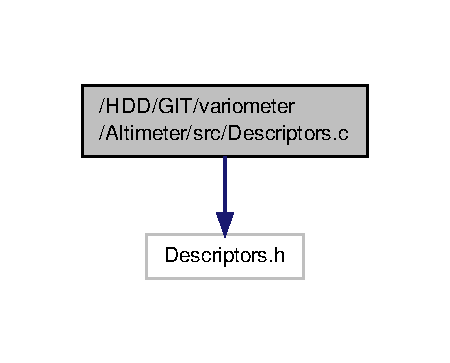
\includegraphics[width=172pt]{_descriptors_8c__incl}
\end{center}
\end{figure}
\subsection*{Függvények}
\begin{DoxyCompactItemize}
\item 
uint16\-\_\-t {\bf C\-A\-L\-L\-B\-A\-C\-K\-\_\-\-U\-S\-B\-\_\-\-Get\-Descriptor} (uint8\-\_\-t corenum, const uint16\-\_\-t w\-Value, const uint8\-\_\-t w\-Index, const void $\ast$$\ast$const Descriptor\-Address)
\end{DoxyCompactItemize}
\subsection*{Változók}
\begin{DoxyCompactItemize}
\item 
U\-S\-B\-\_\-\-Descriptor\-\_\-\-Device\-\_\-t {\bf Device\-Descriptor}
\item 
U\-S\-B\-\_\-\-Descriptor\-\_\-\-Configuration\-\_\-t {\bf Configuration\-Descriptor}
\item 
uint8\-\_\-t {\bf Language\-String} [$\,$]
\item 
U\-S\-B\-\_\-\-Descriptor\-\_\-\-String\-\_\-t $\ast$ {\bf Language\-String\-Ptr} = (U\-S\-B\-\_\-\-Descriptor\-\_\-\-String\-\_\-t $\ast$) {\bf Language\-String}
\item 
uint8\-\_\-t {\bf Manufacturer\-String} [$\,$]
\item 
U\-S\-B\-\_\-\-Descriptor\-\_\-\-String\-\_\-t $\ast$ {\bf Manufacturer\-String\-Ptr} = (U\-S\-B\-\_\-\-Descriptor\-\_\-\-String\-\_\-t $\ast$) {\bf Manufacturer\-String}
\item 
uint8\-\_\-t {\bf Product\-String} [$\,$]
\item 
U\-S\-B\-\_\-\-Descriptor\-\_\-\-String\-\_\-t $\ast$ {\bf Product\-String\-Ptr} = (U\-S\-B\-\_\-\-Descriptor\-\_\-\-String\-\_\-t $\ast$) {\bf Product\-String}
\end{DoxyCompactItemize}


\subsection{Függvények dokumentációja}
\index{Descriptors.\-c@{Descriptors.\-c}!C\-A\-L\-L\-B\-A\-C\-K\-\_\-\-U\-S\-B\-\_\-\-Get\-Descriptor@{C\-A\-L\-L\-B\-A\-C\-K\-\_\-\-U\-S\-B\-\_\-\-Get\-Descriptor}}
\index{C\-A\-L\-L\-B\-A\-C\-K\-\_\-\-U\-S\-B\-\_\-\-Get\-Descriptor@{C\-A\-L\-L\-B\-A\-C\-K\-\_\-\-U\-S\-B\-\_\-\-Get\-Descriptor}!Descriptors.c@{Descriptors.\-c}}
\subsubsection[{C\-A\-L\-L\-B\-A\-C\-K\-\_\-\-U\-S\-B\-\_\-\-Get\-Descriptor}]{\setlength{\rightskip}{0pt plus 5cm}uint16\-\_\-t C\-A\-L\-L\-B\-A\-C\-K\-\_\-\-U\-S\-B\-\_\-\-Get\-Descriptor (
\begin{DoxyParamCaption}
\item[{uint8\-\_\-t}]{corenum, }
\item[{const uint16\-\_\-t}]{w\-Value, }
\item[{const uint8\-\_\-t}]{w\-Index, }
\item[{const void $\ast$$\ast$const}]{Descriptor\-Address}
\end{DoxyParamCaption}
)}\label{_descriptors_8c_a25529e40317cd4470fae630438b53eff}


Definíció a(z) Descriptors.\-c fájl 250. sorában.



\subsection{Változók dokumentációja}
\index{Descriptors.\-c@{Descriptors.\-c}!Configuration\-Descriptor@{Configuration\-Descriptor}}
\index{Configuration\-Descriptor@{Configuration\-Descriptor}!Descriptors.c@{Descriptors.\-c}}
\subsubsection[{Configuration\-Descriptor}]{\setlength{\rightskip}{0pt plus 5cm}U\-S\-B\-\_\-\-Descriptor\-\_\-\-Configuration\-\_\-t Configuration\-Descriptor}\label{_descriptors_8c_a2d091eefbfaf5bd43f4cf77d140e2d9f}


Definíció a(z) Descriptors.\-c fájl 85. sorában.

\index{Descriptors.\-c@{Descriptors.\-c}!Device\-Descriptor@{Device\-Descriptor}}
\index{Device\-Descriptor@{Device\-Descriptor}!Descriptors.c@{Descriptors.\-c}}
\subsubsection[{Device\-Descriptor}]{\setlength{\rightskip}{0pt plus 5cm}U\-S\-B\-\_\-\-Descriptor\-\_\-\-Device\-\_\-t Device\-Descriptor}\label{_descriptors_8c_a6a373a28a14fd420dd82bdd0f6978544}
{\bfseries Kezdő érték\-:}
\begin{DoxyCode}
= \{
    .Header                 = \{.Size = \textcolor{keyword}{sizeof}(USB\_Descriptor\_Device\_t), .Type = DTYPE\_Device\},

    .USBSpecification       = VERSION\_BCD(01.10),
    .Class                  = CDC\_CSCP\_CDCClass,
    .SubClass               = CDC\_CSCP\_NoSpecificSubclass,
    .Protocol               = CDC\_CSCP\_NoSpecificProtocol,

    .Endpoint0Size          = FIXED\_CONTROL\_ENDPOINT\_SIZE,

    .VendorID               = 0x1fc9,   
    .ProductID              = 0x0083,   
    .ReleaseNumber          = VERSION\_BCD(00.01),

    .ManufacturerStrIndex   = 0x01,
    .ProductStrIndex        = 0x02,
    .SerialNumStrIndex      = USE\_INTERNAL\_SERIAL,

    .NumberOfConfigurations = FIXED\_NUM\_CONFIGURATIONS
\}
\end{DoxyCode}


Definíció a(z) Descriptors.\-c fájl 59. sorában.

\index{Descriptors.\-c@{Descriptors.\-c}!Language\-String@{Language\-String}}
\index{Language\-String@{Language\-String}!Descriptors.c@{Descriptors.\-c}}
\subsubsection[{Language\-String}]{\setlength{\rightskip}{0pt plus 5cm}uint8\-\_\-t Language\-String[$\,$]}\label{_descriptors_8c_a156d44ced236ce8b684a10b2ebb9cd70}
{\bfseries Kezdő érték\-:}
\begin{DoxyCode}
= \{
    USB\_STRING\_LEN(1),
    DTYPE\_String,
    WBVAL(LANGUAGE\_ID\_ENG),
\}
\end{DoxyCode}


Definíció a(z) Descriptors.\-c fájl 188. sorában.

\index{Descriptors.\-c@{Descriptors.\-c}!Language\-String\-Ptr@{Language\-String\-Ptr}}
\index{Language\-String\-Ptr@{Language\-String\-Ptr}!Descriptors.c@{Descriptors.\-c}}
\subsubsection[{Language\-String\-Ptr}]{\setlength{\rightskip}{0pt plus 5cm}U\-S\-B\-\_\-\-Descriptor\-\_\-\-String\-\_\-t$\ast$ Language\-String\-Ptr = (U\-S\-B\-\_\-\-Descriptor\-\_\-\-String\-\_\-t $\ast$) {\bf Language\-String}}\label{_descriptors_8c_a9f3f62928cb9d5d2ca9fbf5eede1cc52}


Definíció a(z) Descriptors.\-c fájl 193. sorában.

\index{Descriptors.\-c@{Descriptors.\-c}!Manufacturer\-String@{Manufacturer\-String}}
\index{Manufacturer\-String@{Manufacturer\-String}!Descriptors.c@{Descriptors.\-c}}
\subsubsection[{Manufacturer\-String}]{\setlength{\rightskip}{0pt plus 5cm}uint8\-\_\-t Manufacturer\-String[$\,$]}\label{_descriptors_8c_af43938f971837cb37b3191312503a7a3}
{\bfseries Kezdő érték\-:}
\begin{DoxyCode}
= \{
    USB\_STRING\_LEN(3),
    DTYPE\_String,
    WBVAL(\textcolor{charliteral}{'N'}),
    WBVAL(\textcolor{charliteral}{'X'}),
    WBVAL(\textcolor{charliteral}{'P'}),
\}
\end{DoxyCode}


Definíció a(z) Descriptors.\-c fájl 199. sorában.

\index{Descriptors.\-c@{Descriptors.\-c}!Manufacturer\-String\-Ptr@{Manufacturer\-String\-Ptr}}
\index{Manufacturer\-String\-Ptr@{Manufacturer\-String\-Ptr}!Descriptors.c@{Descriptors.\-c}}
\subsubsection[{Manufacturer\-String\-Ptr}]{\setlength{\rightskip}{0pt plus 5cm}U\-S\-B\-\_\-\-Descriptor\-\_\-\-String\-\_\-t$\ast$ Manufacturer\-String\-Ptr = (U\-S\-B\-\_\-\-Descriptor\-\_\-\-String\-\_\-t $\ast$) {\bf Manufacturer\-String}}\label{_descriptors_8c_a48338794dea700974f8b0b043d0a4d60}


Definíció a(z) Descriptors.\-c fájl 206. sorában.

\index{Descriptors.\-c@{Descriptors.\-c}!Product\-String@{Product\-String}}
\index{Product\-String@{Product\-String}!Descriptors.c@{Descriptors.\-c}}
\subsubsection[{Product\-String}]{\setlength{\rightskip}{0pt plus 5cm}uint8\-\_\-t Product\-String[$\,$]}\label{_descriptors_8c_afb016d49474419471ed53243c36007f6}
{\bfseries Kezdő érték\-:}
\begin{DoxyCode}
= \{
    USB\_STRING\_LEN(18),
    DTYPE\_String,
    WBVAL(\textcolor{charliteral}{'A'}),
    WBVAL(\textcolor{charliteral}{'l'}),
    WBVAL(\textcolor{charliteral}{'t'}),
    WBVAL(\textcolor{charliteral}{'i'}),
    WBVAL(\textcolor{charliteral}{'m'}),
    WBVAL(\textcolor{charliteral}{'e'}),
    WBVAL(\textcolor{charliteral}{'t'}),
    WBVAL(\textcolor{charliteral}{'e'}),
    WBVAL(\textcolor{charliteral}{'r'}),
    WBVAL(\textcolor{charliteral}{' '}),
    WBVAL(\textcolor{charliteral}{'C'}),
    WBVAL(\textcolor{charliteral}{'D'}),
    WBVAL(\textcolor{charliteral}{'C'}),
    WBVAL(\textcolor{charliteral}{' '}),
    WBVAL(\textcolor{charliteral}{'C'}),
    WBVAL(\textcolor{charliteral}{'o'}),
    WBVAL(\textcolor{charliteral}{'n'}),
    WBVAL(\textcolor{charliteral}{'n'}),
\}
\end{DoxyCode}


Definíció a(z) Descriptors.\-c fájl 212. sorában.

\index{Descriptors.\-c@{Descriptors.\-c}!Product\-String\-Ptr@{Product\-String\-Ptr}}
\index{Product\-String\-Ptr@{Product\-String\-Ptr}!Descriptors.c@{Descriptors.\-c}}
\subsubsection[{Product\-String\-Ptr}]{\setlength{\rightskip}{0pt plus 5cm}U\-S\-B\-\_\-\-Descriptor\-\_\-\-String\-\_\-t$\ast$ Product\-String\-Ptr = (U\-S\-B\-\_\-\-Descriptor\-\_\-\-String\-\_\-t $\ast$) {\bf Product\-String}}\label{_descriptors_8c_aa7a5f39bd07b0c4ded3f6f7f797b1d92}


Definíció a(z) Descriptors.\-c fájl 234. sorában.


\section{/\-H\-D\-D/\-G\-I\-T/variometer/\-Altimeter/src/eeprom.c fájlreferencia}
\label{eeprom_8c}\index{/\-H\-D\-D/\-G\-I\-T/variometer/\-Altimeter/src/eeprom.\-c@{/\-H\-D\-D/\-G\-I\-T/variometer/\-Altimeter/src/eeprom.\-c}}
{\ttfamily \#include \char`\"{}ch.\-h\char`\"{}}\\*
{\ttfamily \#include \char`\"{}hal.\-h\char`\"{}}\\*
{\ttfamily \#include \char`\"{}eeprom.\-h\char`\"{}}\\*
Az eeprom.\-c definíciós fájl függési gráfja\-:
\nopagebreak
\begin{figure}[H]
\begin{center}
\leavevmode
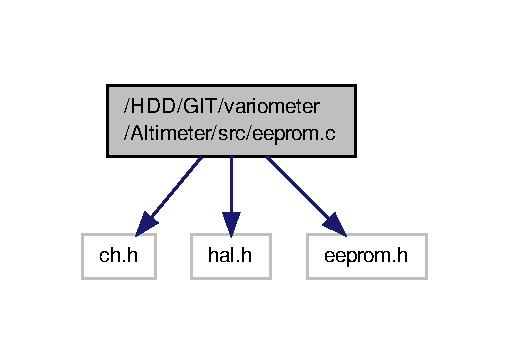
\includegraphics[width=244pt]{eeprom_8c__incl}
\end{center}
\end{figure}
\subsection*{Adatszerkezetek}
\begin{DoxyCompactItemize}
\item 
struct {\bf log\-\_\-rec\-\_\-ext\-\_\-s}
\end{DoxyCompactItemize}
\subsection*{Típusdefiníciók}
\begin{DoxyCompactItemize}
\item 
typedef struct {\bf log\-\_\-rec\-\_\-ext\-\_\-s} {\bf log\-\_\-rec\-\_\-ext\-\_\-t}
\end{DoxyCompactItemize}
\subsection*{Függvények}
\begin{DoxyCompactItemize}
\item 
int {\bf ee\-\_\-write\-\_\-log\-\_\-rec} (log\-\_\-rec\-\_\-t $\ast$record, uint16\-\_\-t $\ast$address)
\begin{DoxyCompactList}\small\item\em Beír egy rekordot az E\-E\-P\-R\-O\-M-\/ba az adott címtől kezdődően. \end{DoxyCompactList}\item 
uint16\-\_\-t {\bf ee\-\_\-read\-\_\-log\-\_\-rec} (log\-\_\-rec\-\_\-t $\ast$record, uint16\-\_\-t from\-\_\-addr, uint16\-\_\-t num\-\_\-of\-\_\-rec)
\begin{DoxyCompactList}\small\item\em Kiolvas adott számú rekordot az E\-E\-P\-R\-O\-M-\/ból az adott címtől kezdődően. \end{DoxyCompactList}\item 
uint16\-\_\-t {\bf ee\-\_\-get\-\_\-first\-\_\-free\-\_\-address} ()
\begin{DoxyCompactList}\small\item\em Visszaadja az első szabad hely címét. \end{DoxyCompactList}\end{DoxyCompactItemize}


\subsection{Típusdefiníciók dokumentációja}
\index{eeprom.\-c@{eeprom.\-c}!log\-\_\-rec\-\_\-ext\-\_\-t@{log\-\_\-rec\-\_\-ext\-\_\-t}}
\index{log\-\_\-rec\-\_\-ext\-\_\-t@{log\-\_\-rec\-\_\-ext\-\_\-t}!eeprom.c@{eeprom.\-c}}
\subsubsection[{log\-\_\-rec\-\_\-ext\-\_\-t}]{\setlength{\rightskip}{0pt plus 5cm}typedef struct {\bf log\-\_\-rec\-\_\-ext\-\_\-s}  {\bf log\-\_\-rec\-\_\-ext\-\_\-t}}\label{eeprom_8c_a87e61d040028e5a92f9169b2dc301095}


\subsection{Függvények dokumentációja}
\index{eeprom.\-c@{eeprom.\-c}!ee\-\_\-get\-\_\-first\-\_\-free\-\_\-address@{ee\-\_\-get\-\_\-first\-\_\-free\-\_\-address}}
\index{ee\-\_\-get\-\_\-first\-\_\-free\-\_\-address@{ee\-\_\-get\-\_\-first\-\_\-free\-\_\-address}!eeprom.c@{eeprom.\-c}}
\subsubsection[{ee\-\_\-get\-\_\-first\-\_\-free\-\_\-address}]{\setlength{\rightskip}{0pt plus 5cm}uint16\-\_\-t ee\-\_\-get\-\_\-first\-\_\-free\-\_\-address (
\begin{DoxyParamCaption}
{}
\end{DoxyParamCaption}
)}\label{eeprom_8c_aa61d5bd2a11169dbd512934b1fb384b7}


Visszaadja az első szabad hely címét. 

\begin{DoxyReturn}{Visszatérési érték}
Az első szabad hely címe az E\-E\-P\-R\-O\-M-\/ban. 
\end{DoxyReturn}


Definíció a(z) eeprom.\-c fájl 140. sorában.



Here is the caller graph for this function\-:
\nopagebreak
\begin{figure}[H]
\begin{center}
\leavevmode
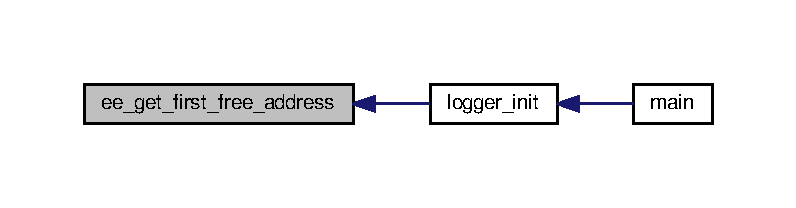
\includegraphics[width=350pt]{eeprom_8c_aa61d5bd2a11169dbd512934b1fb384b7_icgraph}
\end{center}
\end{figure}


\index{eeprom.\-c@{eeprom.\-c}!ee\-\_\-read\-\_\-log\-\_\-rec@{ee\-\_\-read\-\_\-log\-\_\-rec}}
\index{ee\-\_\-read\-\_\-log\-\_\-rec@{ee\-\_\-read\-\_\-log\-\_\-rec}!eeprom.c@{eeprom.\-c}}
\subsubsection[{ee\-\_\-read\-\_\-log\-\_\-rec}]{\setlength{\rightskip}{0pt plus 5cm}uint16\-\_\-t ee\-\_\-read\-\_\-log\-\_\-rec (
\begin{DoxyParamCaption}
\item[{log\-\_\-rec\-\_\-t $\ast$}]{record, }
\item[{uint16\-\_\-t}]{from\-\_\-addr, }
\item[{uint16\-\_\-t}]{num\-\_\-of\-\_\-rec}
\end{DoxyParamCaption}
)}\label{eeprom_8c_a801cca373370aacce8631bd6dfff1373}


Kiolvas adott számú rekordot az E\-E\-P\-R\-O\-M-\/ból az adott címtől kezdődően. 


\begin{DoxyParams}[1]{Paraméterek}
\mbox{\tt out}  & {\em record} & Rekordokból álló tömb, melyet a függvény tölt fel. \\
\hline
\mbox{\tt in}  & {\em from\-\_\-addr} & E\-E\-P\-R\-O\-M cím, ahonnan a kiolvasás kezdődik. \\
\hline
\mbox{\tt in}  & {\em num\-\_\-of\-\_\-rec} & A kiolvasandó rekordok száma. \\
\hline
\end{DoxyParams}
\begin{DoxyReturn}{Visszatérési érték}
A következő kiolvasandó rekord címe. 
\end{DoxyReturn}


Definíció a(z) eeprom.\-c fájl 99. sorában.



Here is the caller graph for this function\-:
\nopagebreak
\begin{figure}[H]
\begin{center}
\leavevmode
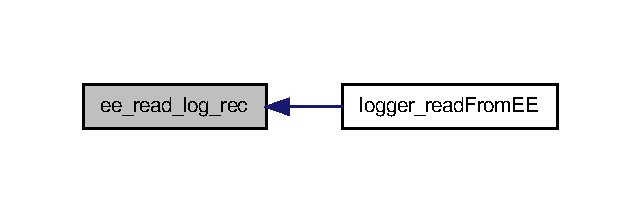
\includegraphics[width=308pt]{eeprom_8c_a801cca373370aacce8631bd6dfff1373_icgraph}
\end{center}
\end{figure}


\index{eeprom.\-c@{eeprom.\-c}!ee\-\_\-write\-\_\-log\-\_\-rec@{ee\-\_\-write\-\_\-log\-\_\-rec}}
\index{ee\-\_\-write\-\_\-log\-\_\-rec@{ee\-\_\-write\-\_\-log\-\_\-rec}!eeprom.c@{eeprom.\-c}}
\subsubsection[{ee\-\_\-write\-\_\-log\-\_\-rec}]{\setlength{\rightskip}{0pt plus 5cm}int ee\-\_\-write\-\_\-log\-\_\-rec (
\begin{DoxyParamCaption}
\item[{log\-\_\-rec\-\_\-t $\ast$}]{record, }
\item[{uint16\-\_\-t $\ast$}]{address}
\end{DoxyParamCaption}
)}\label{eeprom_8c_a601d64b049e61217914cbf9e3c84180a}


Beír egy rekordot az E\-E\-P\-R\-O\-M-\/ba az adott címtől kezdődően. 


\begin{DoxyParams}[1]{Paraméterek}
\mbox{\tt in}  & {\em record} & A beírandó rekord. \\
\hline
\mbox{\tt in}  & {\em address} & E\-E\-P\-R\-O\-M cím, ahová a rekord kerül. \\
\hline
\end{DoxyParams}
\begin{DoxyReturn}{Visszatérési érték}
0 -\/ sikeres, $<$ 0 -\/ sikertelen. 
\end{DoxyReturn}


Definíció a(z) eeprom.\-c fájl 35. sorában.



Here is the caller graph for this function\-:
\nopagebreak
\begin{figure}[H]
\begin{center}
\leavevmode
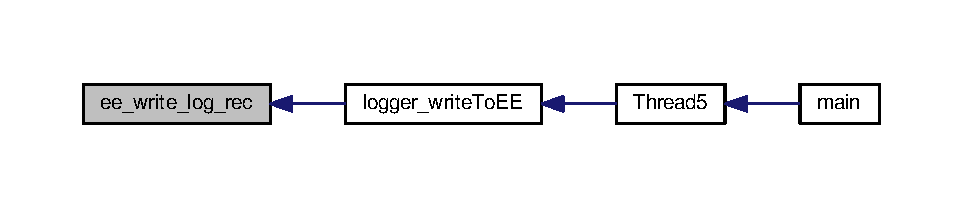
\includegraphics[width=350pt]{eeprom_8c_a601d64b049e61217914cbf9e3c84180a_icgraph}
\end{center}
\end{figure}



\section{/\-H\-D\-D/\-G\-I\-T/variometer/\-Altimeter/src/\-H\-P03.c fájlreferencia}
\label{_h_p03_8c}\index{/\-H\-D\-D/\-G\-I\-T/variometer/\-Altimeter/src/\-H\-P03.\-c@{/\-H\-D\-D/\-G\-I\-T/variometer/\-Altimeter/src/\-H\-P03.\-c}}
{\ttfamily \#include \char`\"{}ch.\-h\char`\"{}}\\*
{\ttfamily \#include \char`\"{}hal.\-h\char`\"{}}\\*
{\ttfamily \#include \char`\"{}H\-P03.\-h\char`\"{}}\\*
{\ttfamily \#include \char`\"{}globals.\-h\char`\"{}}\\*
{\ttfamily \#include $<$string.\-h$>$}\\*
{\ttfamily \#include \char`\"{}mymath.\-h\char`\"{}}\\*
{\ttfamily \#include \char`\"{}Kalman.\-h\char`\"{}}\\*
A H\-P03.\-c definíciós fájl függési gráfja\-:
\nopagebreak
\begin{figure}[H]
\begin{center}
\leavevmode
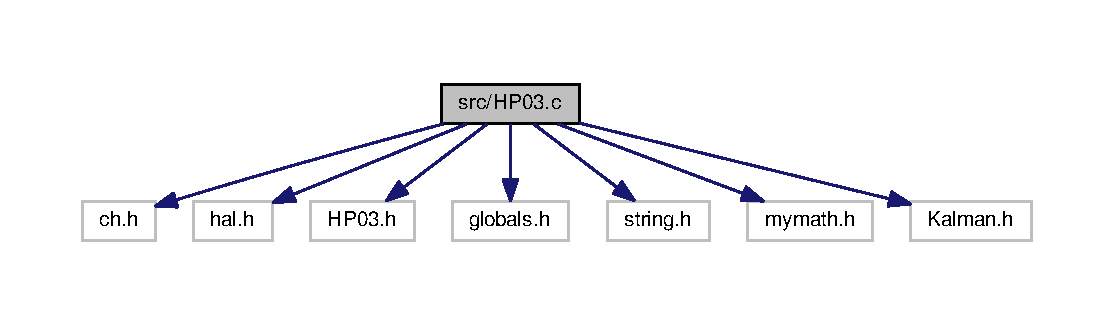
\includegraphics[width=350pt]{_h_p03_8c__incl}
\end{center}
\end{figure}
\subsection*{Függvények}
\begin{DoxyCompactItemize}
\item 
int {\bf H\-P03\-\_\-pressure\-To\-Altitude} (float sea\-Level, H\-P03\-\_\-meas\-\_\-t measured\-Press\-Temp)
\begin{DoxyCompactList}\small\item\em Kiszámítja a magasságot (méterben) a h\-Pa-\/ban megadott légnyomás, tengerszintre átszámított légnyomás és a °\-C-\/ban megadott hőmérséklet alapján. \end{DoxyCompactList}\item 
float {\bf H\-P03\-\_\-pressure\-Sea\-Level\-From\-Altitude} (float altitude, H\-P03\-\_\-meas\-\_\-t measured\-Press\-Temp)
\begin{DoxyCompactList}\small\item\em Kiszámítja a tengerszintre átszámított légnyomást h\-Pa-\/ban az aktuális méterben megadott magasság, h\-Pa-\/ban megadott légnyomás és a °\-C-\/ban megadott hőmérséklet alapján. \end{DoxyCompactList}\item 
void {\bf H\-P03\-\_\-reset} ()
\begin{DoxyCompactList}\small\item\em Alaphelyzetbe állítja a légnyomás szenzort az X\-C\-L\-R kivezetésének alacsony szintre történő álíításával. \end{DoxyCompactList}\item 
void {\bf H\-P03\-\_\-read\-Coeffs} ()
\begin{DoxyCompactList}\small\item\em Kiolvassa a szenzorból a pontos hőmérséklet és légnyomás kiszámításához szükséges koefficiensek értékeit. \end{DoxyCompactList}\item 
int {\bf H\-P03\-\_\-get\-Pressure} (H\-P03\-\_\-meas\-\_\-t $\ast$consts\-In\-\_\-pressure\-Out, bool with\-Kalman)
\begin{DoxyCompactList}\small\item\em Kiolvassa a légnyomás szenzorból a nyomásértéket, majd a koefficiensek segítségével kiszámítja a pontos értéket. \end{DoxyCompactList}\item 
int {\bf H\-P03\-\_\-get\-Temperature} (H\-P03\-\_\-meas\-\_\-t $\ast$result)
\begin{DoxyCompactList}\small\item\em Kiolvassa a légnyomás szenzorból a hőmérsékletet, majd a koefficiensek segítségével kiszámítja a pontos értéket. \end{DoxyCompactList}\end{DoxyCompactItemize}


\subsection{Függvények dokumentációja}
\index{H\-P03.\-c@{H\-P03.\-c}!H\-P03\-\_\-get\-Pressure@{H\-P03\-\_\-get\-Pressure}}
\index{H\-P03\-\_\-get\-Pressure@{H\-P03\-\_\-get\-Pressure}!HP03.c@{H\-P03.\-c}}
\subsubsection[{H\-P03\-\_\-get\-Pressure}]{\setlength{\rightskip}{0pt plus 5cm}int H\-P03\-\_\-get\-Pressure (
\begin{DoxyParamCaption}
\item[{H\-P03\-\_\-meas\-\_\-t $\ast$}]{consts\-In\-\_\-pressure\-Out, }
\item[{bool}]{with\-Kalman}
\end{DoxyParamCaption}
)}\label{_h_p03_8c_a2e206ea1f307f9565982ad14b3582be5}


Kiolvassa a légnyomás szenzorból a nyomásértéket, majd a koefficiensek segítségével kiszámítja a pontos értéket. 


\begin{DoxyParams}[1]{Paraméterek}
\mbox{\tt in,out}  & {\em consts\-In\-\_\-pressure\-Out} & Itt keletkezik az eredmény. \\
\hline
\mbox{\tt in}  & {\em with\-Kalman} & Használja-\/e a Kálmán szűrőt. \\
\hline
\end{DoxyParams}
\begin{DoxyReturn}{Visszatérési érték}
0, ha sikeres. 
\end{DoxyReturn}


Definíció a(z) H\-P03.\-c fájl 150. sorában.



A függvény hívási gráfja\-:
\nopagebreak
\begin{figure}[H]
\begin{center}
\leavevmode
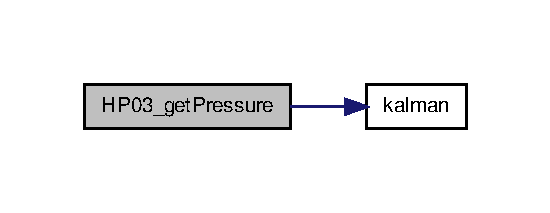
\includegraphics[width=264pt]{_h_p03_8c_a2e206ea1f307f9565982ad14b3582be5_cgraph}
\end{center}
\end{figure}




Here is the caller graph for this function\-:
\nopagebreak
\begin{figure}[H]
\begin{center}
\leavevmode
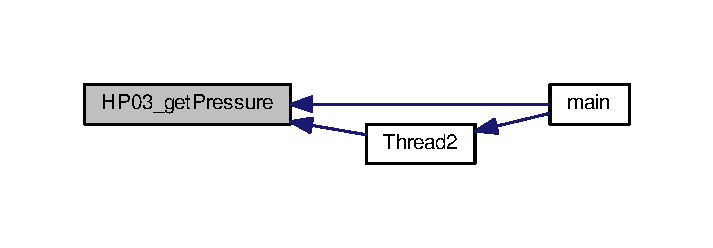
\includegraphics[width=342pt]{_h_p03_8c_a2e206ea1f307f9565982ad14b3582be5_icgraph}
\end{center}
\end{figure}


\index{H\-P03.\-c@{H\-P03.\-c}!H\-P03\-\_\-get\-Temperature@{H\-P03\-\_\-get\-Temperature}}
\index{H\-P03\-\_\-get\-Temperature@{H\-P03\-\_\-get\-Temperature}!HP03.c@{H\-P03.\-c}}
\subsubsection[{H\-P03\-\_\-get\-Temperature}]{\setlength{\rightskip}{0pt plus 5cm}int H\-P03\-\_\-get\-Temperature (
\begin{DoxyParamCaption}
\item[{H\-P03\-\_\-meas\-\_\-t $\ast$}]{result}
\end{DoxyParamCaption}
)}\label{_h_p03_8c_a514dfc9c4a90f039f562c24d6a372486}


Kiolvassa a légnyomás szenzorból a hőmérsékletet, majd a koefficiensek segítségével kiszámítja a pontos értéket. 


\begin{DoxyParams}[1]{Paraméterek}
\mbox{\tt out}  & {\em result} & Itt keletkezik az eredmény. \\
\hline
\end{DoxyParams}
\begin{DoxyReturn}{Visszatérési érték}
0, ha sikeres. 
\end{DoxyReturn}


Definíció a(z) H\-P03.\-c fájl 215. sorában.



Here is the caller graph for this function\-:
\nopagebreak
\begin{figure}[H]
\begin{center}
\leavevmode
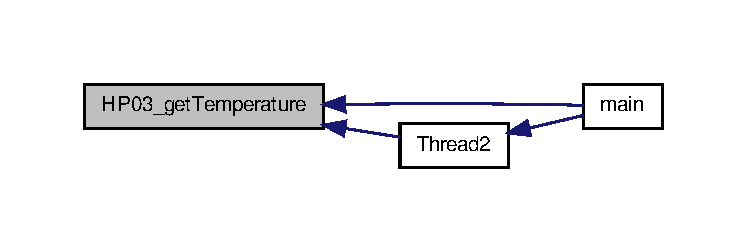
\includegraphics[width=350pt]{_h_p03_8c_a514dfc9c4a90f039f562c24d6a372486_icgraph}
\end{center}
\end{figure}


\index{H\-P03.\-c@{H\-P03.\-c}!H\-P03\-\_\-pressure\-Sea\-Level\-From\-Altitude@{H\-P03\-\_\-pressure\-Sea\-Level\-From\-Altitude}}
\index{H\-P03\-\_\-pressure\-Sea\-Level\-From\-Altitude@{H\-P03\-\_\-pressure\-Sea\-Level\-From\-Altitude}!HP03.c@{H\-P03.\-c}}
\subsubsection[{H\-P03\-\_\-pressure\-Sea\-Level\-From\-Altitude}]{\setlength{\rightskip}{0pt plus 5cm}float H\-P03\-\_\-pressure\-Sea\-Level\-From\-Altitude (
\begin{DoxyParamCaption}
\item[{float}]{altitude, }
\item[{H\-P03\-\_\-meas\-\_\-t}]{measured\-Press\-Temp}
\end{DoxyParamCaption}
)}\label{_h_p03_8c_a1013cdcfcdf48995025d9d2cf1778794}


Kiszámítja a tengerszintre átszámított légnyomást h\-Pa-\/ban az aktuális méterben megadott magasság, h\-Pa-\/ban megadott légnyomás és a °\-C-\/ban megadott hőmérséklet alapján. 


\begin{DoxyParams}[1]{Paraméterek}
\mbox{\tt in}  & {\em altitude} & Magasság méterben. \\
\hline
\mbox{\tt in}  & {\em measured\-Press\-Temp} & Mért légnyomás és hőmérséklet. \\
\hline
\end{DoxyParams}
\begin{DoxyReturn}{Visszatérési érték}
Tengerszintre átszámított légnyomás h\-Pa-\/ban. 
\end{DoxyReturn}


Definíció a(z) H\-P03.\-c fájl 71. sorában.



A függvény hívási gráfja\-:
\nopagebreak
\begin{figure}[H]
\begin{center}
\leavevmode
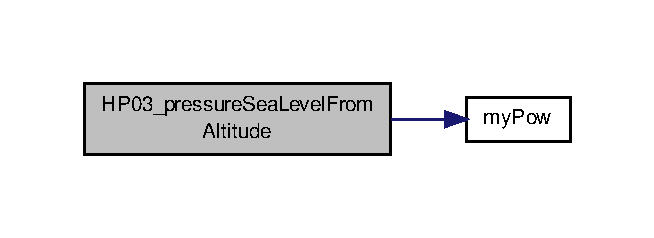
\includegraphics[width=314pt]{_h_p03_8c_a1013cdcfcdf48995025d9d2cf1778794_cgraph}
\end{center}
\end{figure}




Here is the caller graph for this function\-:
\nopagebreak
\begin{figure}[H]
\begin{center}
\leavevmode
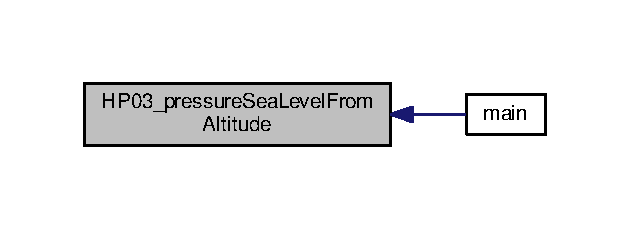
\includegraphics[width=302pt]{_h_p03_8c_a1013cdcfcdf48995025d9d2cf1778794_icgraph}
\end{center}
\end{figure}


\index{H\-P03.\-c@{H\-P03.\-c}!H\-P03\-\_\-pressure\-To\-Altitude@{H\-P03\-\_\-pressure\-To\-Altitude}}
\index{H\-P03\-\_\-pressure\-To\-Altitude@{H\-P03\-\_\-pressure\-To\-Altitude}!HP03.c@{H\-P03.\-c}}
\subsubsection[{H\-P03\-\_\-pressure\-To\-Altitude}]{\setlength{\rightskip}{0pt plus 5cm}int H\-P03\-\_\-pressure\-To\-Altitude (
\begin{DoxyParamCaption}
\item[{float}]{sea\-Level, }
\item[{H\-P03\-\_\-meas\-\_\-t}]{measured\-Press\-Temp}
\end{DoxyParamCaption}
)}\label{_h_p03_8c_a212fee37479d1b104e74f33ccfaab106}


Kiszámítja a magasságot (méterben) a h\-Pa-\/ban megadott légnyomás, tengerszintre átszámított légnyomás és a °\-C-\/ban megadott hőmérséklet alapján. 


\begin{DoxyParams}[1]{Paraméterek}
\mbox{\tt in}  & {\em sea\-Level} & Tengerszintre átszámított légnyomás h\-Pa-\/ban. \\
\hline
\mbox{\tt in}  & {\em measured\-Press\-Temp} & Mért légnyomás és hőmérséklet. \\
\hline
\end{DoxyParams}
\begin{DoxyReturn}{Visszatérési érték}
Magasság méterben. 
\end{DoxyReturn}


Definíció a(z) H\-P03.\-c fájl 40. sorában.



A függvény hívási gráfja\-:
\nopagebreak
\begin{figure}[H]
\begin{center}
\leavevmode
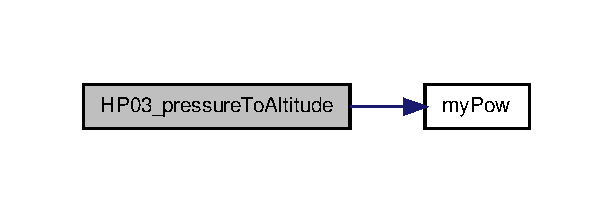
\includegraphics[width=294pt]{_h_p03_8c_a212fee37479d1b104e74f33ccfaab106_cgraph}
\end{center}
\end{figure}




Here is the caller graph for this function\-:
\nopagebreak
\begin{figure}[H]
\begin{center}
\leavevmode
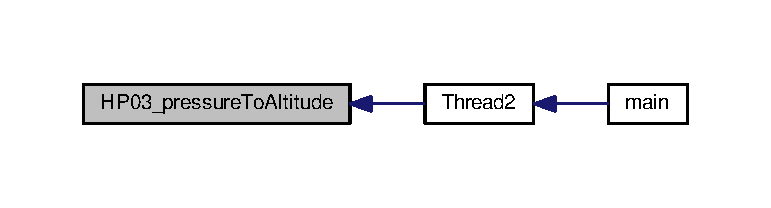
\includegraphics[width=350pt]{_h_p03_8c_a212fee37479d1b104e74f33ccfaab106_icgraph}
\end{center}
\end{figure}


\index{H\-P03.\-c@{H\-P03.\-c}!H\-P03\-\_\-read\-Coeffs@{H\-P03\-\_\-read\-Coeffs}}
\index{H\-P03\-\_\-read\-Coeffs@{H\-P03\-\_\-read\-Coeffs}!HP03.c@{H\-P03.\-c}}
\subsubsection[{H\-P03\-\_\-read\-Coeffs}]{\setlength{\rightskip}{0pt plus 5cm}void H\-P03\-\_\-read\-Coeffs (
\begin{DoxyParamCaption}
{}
\end{DoxyParamCaption}
)}\label{_h_p03_8c_a8b6f09ca977f999dfc96f1c355713bab}


Kiolvassa a szenzorból a pontos hőmérséklet és légnyomás kiszámításához szükséges koefficiensek értékeit. 

\begin{DoxyReturn}{Visszatérési érték}
H\-P03\-\_\-coeff változó. 
\end{DoxyReturn}


Definíció a(z) H\-P03.\-c fájl 116. sorában.



Here is the caller graph for this function\-:
\nopagebreak
\begin{figure}[H]
\begin{center}
\leavevmode
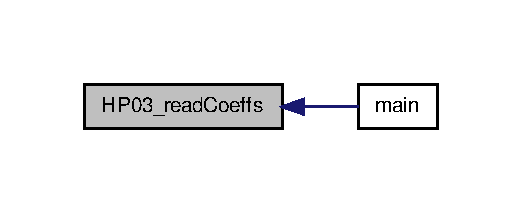
\includegraphics[width=250pt]{_h_p03_8c_a8b6f09ca977f999dfc96f1c355713bab_icgraph}
\end{center}
\end{figure}


\index{H\-P03.\-c@{H\-P03.\-c}!H\-P03\-\_\-reset@{H\-P03\-\_\-reset}}
\index{H\-P03\-\_\-reset@{H\-P03\-\_\-reset}!HP03.c@{H\-P03.\-c}}
\subsubsection[{H\-P03\-\_\-reset}]{\setlength{\rightskip}{0pt plus 5cm}void H\-P03\-\_\-reset (
\begin{DoxyParamCaption}
{}
\end{DoxyParamCaption}
)}\label{_h_p03_8c_a20b369f3261a05f3049139a070607b6d}


Alaphelyzetbe állítja a légnyomás szenzort az X\-C\-L\-R kivezetésének alacsony szintre történő álíításával. 



Definíció a(z) H\-P03.\-c fájl 101. sorában.



Here is the caller graph for this function\-:
\nopagebreak
\begin{figure}[H]
\begin{center}
\leavevmode
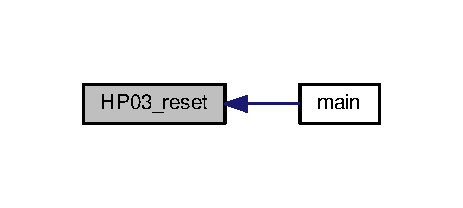
\includegraphics[width=222pt]{_h_p03_8c_a20b369f3261a05f3049139a070607b6d_icgraph}
\end{center}
\end{figure}



\section{/\-H\-D\-D/\-G\-I\-T/variometer/\-Altimeter/src/itoa.c fájlreferencia}
\label{itoa_8c}\index{/\-H\-D\-D/\-G\-I\-T/variometer/\-Altimeter/src/itoa.\-c@{/\-H\-D\-D/\-G\-I\-T/variometer/\-Altimeter/src/itoa.\-c}}
{\ttfamily \#include \char`\"{}itoa.\-h\char`\"{}}\\*
Az itoa.\-c definíciós fájl függési gráfja\-:
\nopagebreak
\begin{figure}[H]
\begin{center}
\leavevmode
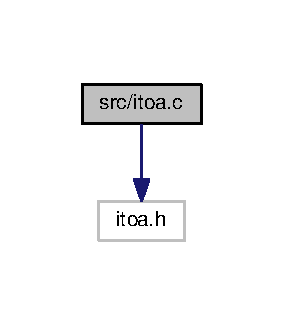
\includegraphics[width=190pt]{itoa_8c__incl}
\end{center}
\end{figure}
\subsection*{Függvények}
\begin{DoxyCompactItemize}
\item 
char $\ast$ {\bf itoa} (int value, char $\ast$buffer, int base, int decimals, int expected\-Length, char padding\-\_\-char, char $\ast$prefix, char $\ast$suffix)
\begin{DoxyCompactList}\small\item\em Előjeles egészet karakter tömbbé konvertál. \end{DoxyCompactList}\end{DoxyCompactItemize}


\subsection{Függvények dokumentációja}
\index{itoa.\-c@{itoa.\-c}!itoa@{itoa}}
\index{itoa@{itoa}!itoa.c@{itoa.\-c}}
\subsubsection[{itoa}]{\setlength{\rightskip}{0pt plus 5cm}char$\ast$ itoa (
\begin{DoxyParamCaption}
\item[{int}]{value, }
\item[{char $\ast$}]{buffer, }
\item[{int}]{base, }
\item[{int}]{decimals, }
\item[{int}]{expected\-Length, }
\item[{char}]{padding\-\_\-char, }
\item[{char $\ast$}]{prefix, }
\item[{char $\ast$}]{suffix}
\end{DoxyParamCaption}
)}\label{itoa_8c_ad140b3216ed9e7c8a084acc96dbd5678}


Előjeles egészet karakter tömbbé konvertál. 


\begin{DoxyParams}[1]{Paraméterek}
\mbox{\tt in}  & {\em value} & Az átalakítandó egész szám. \\
\hline
\mbox{\tt out}  & {\em buffer} & Itt keletkezik az eredmény. \\
\hline
\mbox{\tt in}  & {\em base} & Alap (2; 10; 16 lehet). \\
\hline
\mbox{\tt in}  & {\em decimals} & Tizedesek száma. \\
\hline
\mbox{\tt in}  & {\em expected\-Length} & Kívánt karakterhosszúság. \\
\hline
\mbox{\tt in}  & {\em padding\-\_\-char} & Kitöltő karakter. \\
\hline
\mbox{\tt in}  & {\em prefix} & Előtag, mely a karakterlánc elejéhez fűződik. \\
\hline
\mbox{\tt in}  & {\em suffix} & Utótag, mely a karakterlánc végéhez fűződik. \\
\hline
\end{DoxyParams}
\begin{DoxyReturn}{Visszatérési érték}
Mutató az eredmény bufferre. 
\end{DoxyReturn}


Definíció a(z) itoa.\-c fájl 28. sorában.



Here is the caller graph for this function\-:
\nopagebreak
\begin{figure}[H]
\begin{center}
\leavevmode
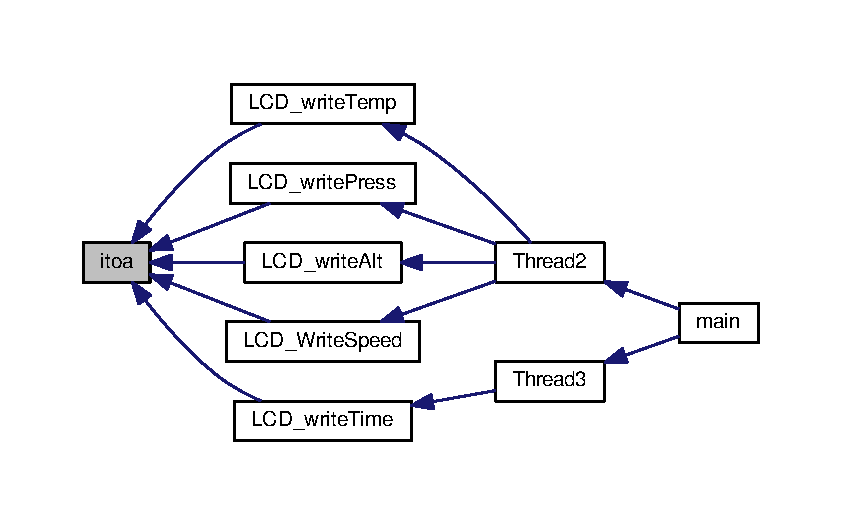
\includegraphics[width=350pt]{itoa_8c_ad140b3216ed9e7c8a084acc96dbd5678_icgraph}
\end{center}
\end{figure}



\section{src/\-Kalman.c fájlreferencia}
\label{_kalman_8c}\index{src/\-Kalman.\-c@{src/\-Kalman.\-c}}
{\ttfamily \#include \char`\"{}Kalman.\-h\char`\"{}}\\*
A Kalman.\-c definíciós fájl függési gráfja\-:
\nopagebreak
\begin{figure}[H]
\begin{center}
\leavevmode
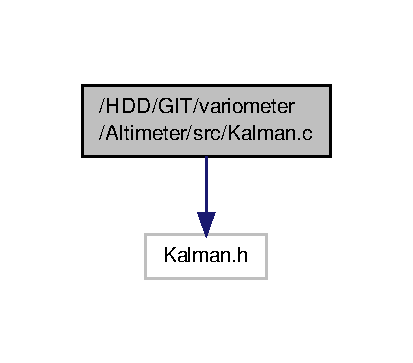
\includegraphics[width=154pt]{_kalman_8c__incl}
\end{center}
\end{figure}
\subsection*{Függvények}
\begin{DoxyCompactItemize}
\item 
void {\bf init\-\_\-kalman} (int z\-\_\-measured)
\begin{DoxyCompactList}\small\item\em A Kálmán szűrő inicializálása. \end{DoxyCompactList}\item 
int {\bf kalman} (int z\-\_\-measured)
\begin{DoxyCompactList}\small\item\em Elvégzi a szűrést (jóslás, erősítés, korrekció). \end{DoxyCompactList}\end{DoxyCompactItemize}


\subsection{Függvények dokumentációja}
\index{Kalman.\-c@{Kalman.\-c}!init\-\_\-kalman@{init\-\_\-kalman}}
\index{init\-\_\-kalman@{init\-\_\-kalman}!Kalman.c@{Kalman.\-c}}
\subsubsection[{init\-\_\-kalman}]{\setlength{\rightskip}{0pt plus 5cm}void init\-\_\-kalman (
\begin{DoxyParamCaption}
\item[{int}]{z\-\_\-measured}
\end{DoxyParamCaption}
)}\label{_kalman_8c_a6ff19aa3f59897d3931e2d728eb37b50}


A Kálmán szűrő inicializálása. 


\begin{DoxyParams}[1]{Paraméterek}
\mbox{\tt in}  & {\em z\-\_\-measured} & A mért érték. \\
\hline
\end{DoxyParams}


Definíció a(z) Kalman.\-c fájl 23. sorában.



Here is the caller graph for this function\-:
\nopagebreak
\begin{figure}[H]
\begin{center}
\leavevmode
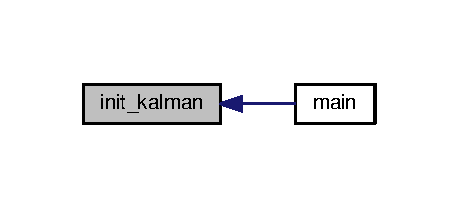
\includegraphics[width=220pt]{_kalman_8c_a6ff19aa3f59897d3931e2d728eb37b50_icgraph}
\end{center}
\end{figure}


\index{Kalman.\-c@{Kalman.\-c}!kalman@{kalman}}
\index{kalman@{kalman}!Kalman.c@{Kalman.\-c}}
\subsubsection[{kalman}]{\setlength{\rightskip}{0pt plus 5cm}int kalman (
\begin{DoxyParamCaption}
\item[{int}]{z\-\_\-measured}
\end{DoxyParamCaption}
)}\label{_kalman_8c_a805a67ac627b7712612544e1c006b12d}


Elvégzi a szűrést (jóslás, erősítés, korrekció). 


\begin{DoxyParams}[1]{Paraméterek}
\mbox{\tt in}  & {\em z\-\_\-measured} & A mért érték. \\
\hline
\end{DoxyParams}
\begin{DoxyReturn}{Visszatérési érték}
Számított (jósolt) érték. 
\end{DoxyReturn}
$<$ Jóslás

$<$ Kálmán erősítés számítása

$<$ Korrekció

Utolsó érték frissítése 

Definíció a(z) Kalman.\-c fájl 33. sorában.



Here is the caller graph for this function\-:
\nopagebreak
\begin{figure}[H]
\begin{center}
\leavevmode
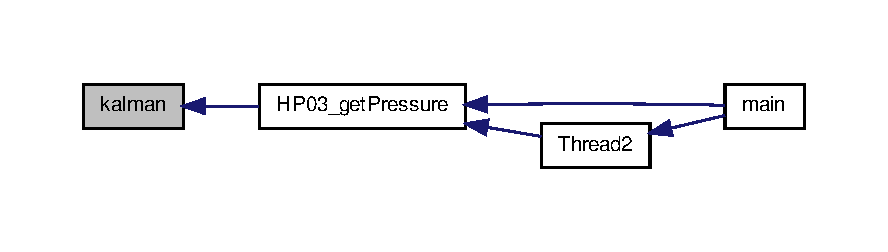
\includegraphics[width=350pt]{_kalman_8c_a805a67ac627b7712612544e1c006b12d_icgraph}
\end{center}
\end{figure}



\section{src/\-L\-C\-D.c fájlreferencia}
\label{_l_c_d_8c}\index{src/\-L\-C\-D.\-c@{src/\-L\-C\-D.\-c}}
{\ttfamily \#include \char`\"{}ch.\-h\char`\"{}}\\*
{\ttfamily \#include \char`\"{}hal.\-h\char`\"{}}\\*
{\ttfamily \#include \char`\"{}L\-C\-D.\-h\char`\"{}}\\*
{\ttfamily \#include \char`\"{}L\-C\-D\-\_\-fonts.\-h\char`\"{}}\\*
{\ttfamily \#include \char`\"{}globals.\-h\char`\"{}}\\*
A L\-C\-D.\-c definíciós fájl függési gráfja\-:
\nopagebreak
\begin{figure}[H]
\begin{center}
\leavevmode
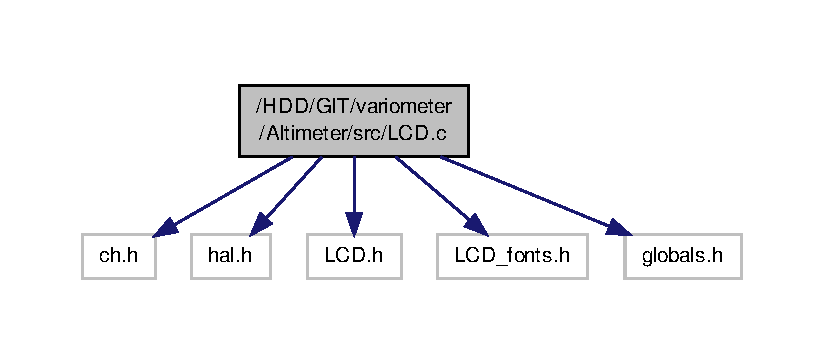
\includegraphics[width=350pt]{_l_c_d_8c__incl}
\end{center}
\end{figure}
\subsection*{Függvények}
\begin{DoxyCompactItemize}
\item 
void {\bf L\-C\-D\-\_\-clear} ()
\begin{DoxyCompactList}\small\item\em Törli a kijelző tartalmát. \end{DoxyCompactList}\item 
void {\bf L\-C\-D\-\_\-init} ()
\begin{DoxyCompactList}\small\item\em A kijelző inicializálását végzi. \end{DoxyCompactList}\item 
void {\bf L\-C\-D\-\_\-write\-Temp} (H\-P03\-\_\-meas\-\_\-t measured\-By\-H\-P03)
\begin{DoxyCompactList}\small\item\em Hőmérséklet megjelenítése a kijelzőn. \end{DoxyCompactList}\item 
void {\bf L\-C\-D\-\_\-write\-Press} (H\-P03\-\_\-meas\-\_\-t measured\-By\-H\-P03)
\begin{DoxyCompactList}\small\item\em Légnyomás megjelenítése a kijelzőn. \end{DoxyCompactList}\item 
void {\bf L\-C\-D\-\_\-write\-Alt} (int alt\-To\-Write)
\begin{DoxyCompactList}\small\item\em Magasság megjelenítése a kijelzőn. \end{DoxyCompactList}\item 
void {\bf L\-C\-D\-\_\-write\-Date} (R\-T\-C\-\_\-date\-\_\-t date\-To\-Write)
\begin{DoxyCompactList}\small\item\em Dátum megjelenítése a kijelzőn. \end{DoxyCompactList}\item 
void {\bf L\-C\-D\-\_\-write\-Time} (R\-T\-C\-\_\-time\-\_\-t time\-To\-Write)
\begin{DoxyCompactList}\small\item\em Idő megjelenítése a kijelzőn. \end{DoxyCompactList}\item 
void {\bf L\-C\-D\-\_\-write\-U\-S\-B} ()
\begin{DoxyCompactList}\small\item\em U\-S\-B felirat megjelenítése a kijelzőn. \end{DoxyCompactList}\item 
void {\bf L\-C\-D\-\_\-write\-U\-S\-B\-\_\-delete} ()
\begin{DoxyCompactList}\small\item\em U\-S\-B felirat törlése a kijelzőről. \end{DoxyCompactList}\item 
void {\bf L\-C\-D\-\_\-write\-L\-O\-G} ()
\begin{DoxyCompactList}\small\item\em L\-O\-G felirat megjelenítése a kijelzőn. \end{DoxyCompactList}\item 
void {\bf L\-C\-D\-\_\-write\-L\-O\-G\-\_\-delete} ()
\begin{DoxyCompactList}\small\item\em L\-O\-G felirat törlése a kijelzőről. \end{DoxyCompactList}\item 
void {\bf L\-C\-D\-\_\-\-Write\-Speed} (int prev\-Alt, int act\-Alt, int delta\-Time)
\begin{DoxyCompactList}\small\item\em A függőleges sebesség megjelenítése a kijelzőn. \end{DoxyCompactList}\end{DoxyCompactItemize}


\subsection{Függvények dokumentációja}
\index{L\-C\-D.\-c@{L\-C\-D.\-c}!L\-C\-D\-\_\-clear@{L\-C\-D\-\_\-clear}}
\index{L\-C\-D\-\_\-clear@{L\-C\-D\-\_\-clear}!LCD.c@{L\-C\-D.\-c}}
\subsubsection[{L\-C\-D\-\_\-clear}]{\setlength{\rightskip}{0pt plus 5cm}void L\-C\-D\-\_\-clear (
\begin{DoxyParamCaption}
{}
\end{DoxyParamCaption}
)}\label{_l_c_d_8c_abe38d05e225c701bebf5a61201331a85}


Törli a kijelző tartalmát. 



Definíció a(z) L\-C\-D.\-c fájl 148. sorában.



Here is the caller graph for this function\-:
\nopagebreak
\begin{figure}[H]
\begin{center}
\leavevmode
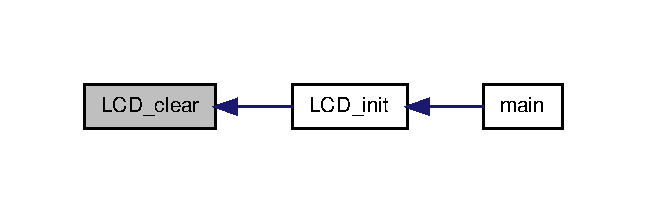
\includegraphics[width=310pt]{_l_c_d_8c_abe38d05e225c701bebf5a61201331a85_icgraph}
\end{center}
\end{figure}


\index{L\-C\-D.\-c@{L\-C\-D.\-c}!L\-C\-D\-\_\-init@{L\-C\-D\-\_\-init}}
\index{L\-C\-D\-\_\-init@{L\-C\-D\-\_\-init}!LCD.c@{L\-C\-D.\-c}}
\subsubsection[{L\-C\-D\-\_\-init}]{\setlength{\rightskip}{0pt plus 5cm}void L\-C\-D\-\_\-init (
\begin{DoxyParamCaption}
{}
\end{DoxyParamCaption}
)}\label{_l_c_d_8c_a0742e25c23ca1096ceba081b98fd58ba}


A kijelző inicializálását végzi. 

$<$ Power\-O\-N, Ext\-Command\-Set -\/ 0x21

$<$ Internal H\-V-\/gen x3 -\/ 0x09

$<$ Set Vop

$<$ Bias n=2

$<$ Temperature coeff 2

$<$ Standart\-Command\-Set -\/ 0x20

$<$ normal mode, display non-\/inverted 

Definíció a(z) L\-C\-D.\-c fájl 169. sorában.



A függvény hívási gráfja\-:\nopagebreak
\begin{figure}[H]
\begin{center}
\leavevmode
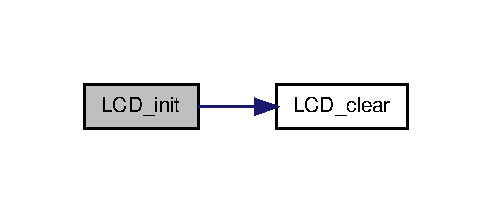
\includegraphics[width=236pt]{_l_c_d_8c_a0742e25c23ca1096ceba081b98fd58ba_cgraph}
\end{center}
\end{figure}




Here is the caller graph for this function\-:
\nopagebreak
\begin{figure}[H]
\begin{center}
\leavevmode
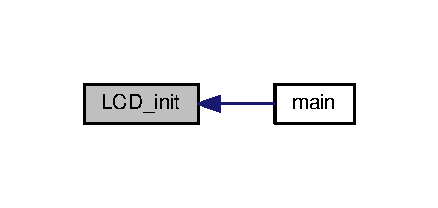
\includegraphics[width=210pt]{_l_c_d_8c_a0742e25c23ca1096ceba081b98fd58ba_icgraph}
\end{center}
\end{figure}


\index{L\-C\-D.\-c@{L\-C\-D.\-c}!L\-C\-D\-\_\-write\-Alt@{L\-C\-D\-\_\-write\-Alt}}
\index{L\-C\-D\-\_\-write\-Alt@{L\-C\-D\-\_\-write\-Alt}!LCD.c@{L\-C\-D.\-c}}
\subsubsection[{L\-C\-D\-\_\-write\-Alt}]{\setlength{\rightskip}{0pt plus 5cm}void L\-C\-D\-\_\-write\-Alt (
\begin{DoxyParamCaption}
\item[{int}]{alt\-To\-Write}
\end{DoxyParamCaption}
)}\label{_l_c_d_8c_a4f21373ce23ee38fa023546e0b262fdf}


Magasság megjelenítése a kijelzőn. 


\begin{DoxyParams}[1]{Paraméterek}
\mbox{\tt in}  & {\em alt\-To\-Write} & Magasság érték. \\
\hline
\end{DoxyParams}


Definíció a(z) L\-C\-D.\-c fájl 250. sorában.



A függvény hívási gráfja\-:\nopagebreak
\begin{figure}[H]
\begin{center}
\leavevmode
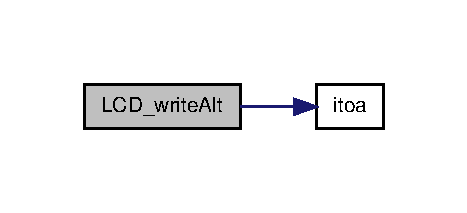
\includegraphics[width=224pt]{_l_c_d_8c_a4f21373ce23ee38fa023546e0b262fdf_cgraph}
\end{center}
\end{figure}




Here is the caller graph for this function\-:
\nopagebreak
\begin{figure}[H]
\begin{center}
\leavevmode
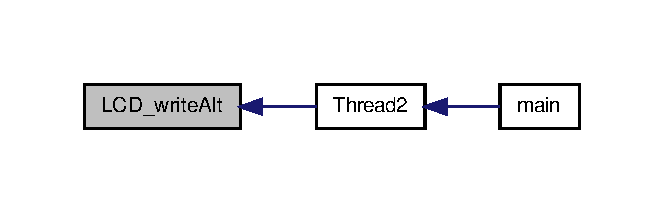
\includegraphics[width=318pt]{_l_c_d_8c_a4f21373ce23ee38fa023546e0b262fdf_icgraph}
\end{center}
\end{figure}


\index{L\-C\-D.\-c@{L\-C\-D.\-c}!L\-C\-D\-\_\-write\-Date@{L\-C\-D\-\_\-write\-Date}}
\index{L\-C\-D\-\_\-write\-Date@{L\-C\-D\-\_\-write\-Date}!LCD.c@{L\-C\-D.\-c}}
\subsubsection[{L\-C\-D\-\_\-write\-Date}]{\setlength{\rightskip}{0pt plus 5cm}void L\-C\-D\-\_\-write\-Date (
\begin{DoxyParamCaption}
\item[{R\-T\-C\-\_\-date\-\_\-t}]{date\-To\-Write}
\end{DoxyParamCaption}
)}\label{_l_c_d_8c_adfcdedfb3a022310629af2dc94a1f658}


Dátum megjelenítése a kijelzőn. 


\begin{DoxyParams}[1]{Paraméterek}
\mbox{\tt in}  & {\em date\-To\-Write} & Dátum érték. \\
\hline
\end{DoxyParams}


Definíció a(z) L\-C\-D.\-c fájl 267. sorában.

\index{L\-C\-D.\-c@{L\-C\-D.\-c}!L\-C\-D\-\_\-write\-L\-O\-G@{L\-C\-D\-\_\-write\-L\-O\-G}}
\index{L\-C\-D\-\_\-write\-L\-O\-G@{L\-C\-D\-\_\-write\-L\-O\-G}!LCD.c@{L\-C\-D.\-c}}
\subsubsection[{L\-C\-D\-\_\-write\-L\-O\-G}]{\setlength{\rightskip}{0pt plus 5cm}void L\-C\-D\-\_\-write\-L\-O\-G (
\begin{DoxyParamCaption}
{}
\end{DoxyParamCaption}
)}\label{_l_c_d_8c_a86cd2b845f3f477af8997fd140746759}


L\-O\-G felirat megjelenítése a kijelzőn. 



Definíció a(z) L\-C\-D.\-c fájl 333. sorában.



Here is the caller graph for this function\-:
\nopagebreak
\begin{figure}[H]
\begin{center}
\leavevmode
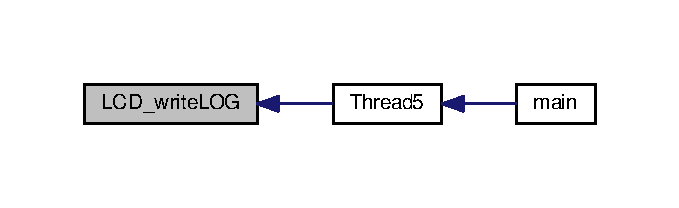
\includegraphics[width=326pt]{_l_c_d_8c_a86cd2b845f3f477af8997fd140746759_icgraph}
\end{center}
\end{figure}


\index{L\-C\-D.\-c@{L\-C\-D.\-c}!L\-C\-D\-\_\-write\-L\-O\-G\-\_\-delete@{L\-C\-D\-\_\-write\-L\-O\-G\-\_\-delete}}
\index{L\-C\-D\-\_\-write\-L\-O\-G\-\_\-delete@{L\-C\-D\-\_\-write\-L\-O\-G\-\_\-delete}!LCD.c@{L\-C\-D.\-c}}
\subsubsection[{L\-C\-D\-\_\-write\-L\-O\-G\-\_\-delete}]{\setlength{\rightskip}{0pt plus 5cm}void L\-C\-D\-\_\-write\-L\-O\-G\-\_\-delete (
\begin{DoxyParamCaption}
{}
\end{DoxyParamCaption}
)}\label{_l_c_d_8c_a7f475dedd89b9b5b3b961dbc096d052a}


L\-O\-G felirat törlése a kijelzőről. 



Definíció a(z) L\-C\-D.\-c fájl 346. sorában.



Here is the caller graph for this function\-:
\nopagebreak
\begin{figure}[H]
\begin{center}
\leavevmode
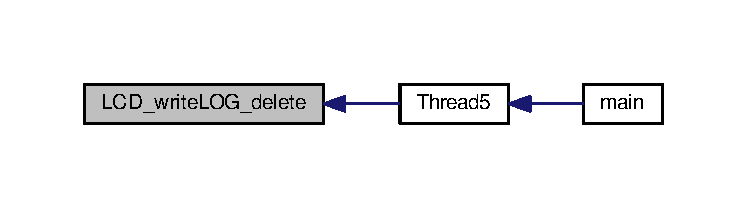
\includegraphics[width=350pt]{_l_c_d_8c_a7f475dedd89b9b5b3b961dbc096d052a_icgraph}
\end{center}
\end{figure}


\index{L\-C\-D.\-c@{L\-C\-D.\-c}!L\-C\-D\-\_\-write\-Press@{L\-C\-D\-\_\-write\-Press}}
\index{L\-C\-D\-\_\-write\-Press@{L\-C\-D\-\_\-write\-Press}!LCD.c@{L\-C\-D.\-c}}
\subsubsection[{L\-C\-D\-\_\-write\-Press}]{\setlength{\rightskip}{0pt plus 5cm}void L\-C\-D\-\_\-write\-Press (
\begin{DoxyParamCaption}
\item[{H\-P03\-\_\-meas\-\_\-t}]{measured\-By\-H\-P03}
\end{DoxyParamCaption}
)}\label{_l_c_d_8c_a66c85acb573ef9bcfa2ae5f95feb596f}


Légnyomás megjelenítése a kijelzőn. 


\begin{DoxyParams}[1]{Paraméterek}
\mbox{\tt in}  & {\em measured\-By\-H\-P03} & Nyomás érték. \\
\hline
\end{DoxyParams}


Definíció a(z) L\-C\-D.\-c fájl 225. sorában.



A függvény hívási gráfja\-:\nopagebreak
\begin{figure}[H]
\begin{center}
\leavevmode
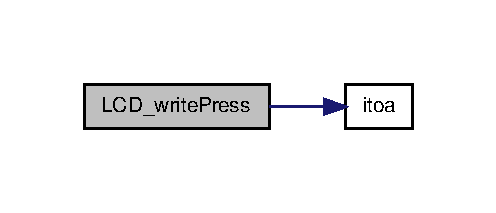
\includegraphics[width=238pt]{_l_c_d_8c_a66c85acb573ef9bcfa2ae5f95feb596f_cgraph}
\end{center}
\end{figure}




Here is the caller graph for this function\-:
\nopagebreak
\begin{figure}[H]
\begin{center}
\leavevmode
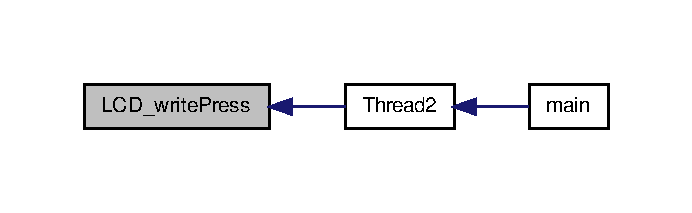
\includegraphics[width=332pt]{_l_c_d_8c_a66c85acb573ef9bcfa2ae5f95feb596f_icgraph}
\end{center}
\end{figure}


\index{L\-C\-D.\-c@{L\-C\-D.\-c}!L\-C\-D\-\_\-\-Write\-Speed@{L\-C\-D\-\_\-\-Write\-Speed}}
\index{L\-C\-D\-\_\-\-Write\-Speed@{L\-C\-D\-\_\-\-Write\-Speed}!LCD.c@{L\-C\-D.\-c}}
\subsubsection[{L\-C\-D\-\_\-\-Write\-Speed}]{\setlength{\rightskip}{0pt plus 5cm}void L\-C\-D\-\_\-\-Write\-Speed (
\begin{DoxyParamCaption}
\item[{int}]{prev\-Alt, }
\item[{int}]{act\-Alt, }
\item[{int}]{delta\-Time}
\end{DoxyParamCaption}
)}\label{_l_c_d_8c_ab1c412a381f9f4fe0668c795010004d1}


A függőleges sebesség megjelenítése a kijelzőn. 


\begin{DoxyParams}[1]{Paraméterek}
\mbox{\tt in}  & {\em prev\-Alt} & Az előző magasság értéke. \\
\hline
\mbox{\tt in}  & {\em act\-Alt} & Az aktuális magasság értéke. \\
\hline
\mbox{\tt in}  & {\em delta\-Time} & A két mérés közt eltelt idő. \\
\hline
\end{DoxyParams}


Definíció a(z) L\-C\-D.\-c fájl 362. sorában.



A függvény hívási gráfja\-:
\nopagebreak
\begin{figure}[H]
\begin{center}
\leavevmode
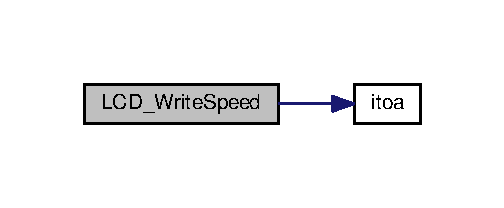
\includegraphics[width=242pt]{_l_c_d_8c_ab1c412a381f9f4fe0668c795010004d1_cgraph}
\end{center}
\end{figure}




Here is the caller graph for this function\-:
\nopagebreak
\begin{figure}[H]
\begin{center}
\leavevmode
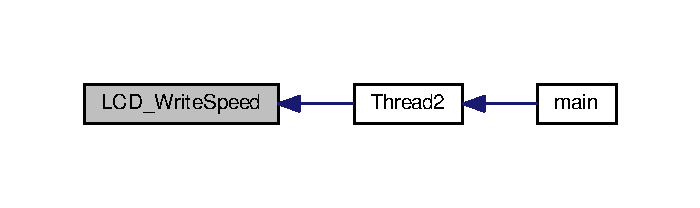
\includegraphics[width=336pt]{_l_c_d_8c_ab1c412a381f9f4fe0668c795010004d1_icgraph}
\end{center}
\end{figure}


\index{L\-C\-D.\-c@{L\-C\-D.\-c}!L\-C\-D\-\_\-write\-Temp@{L\-C\-D\-\_\-write\-Temp}}
\index{L\-C\-D\-\_\-write\-Temp@{L\-C\-D\-\_\-write\-Temp}!LCD.c@{L\-C\-D.\-c}}
\subsubsection[{L\-C\-D\-\_\-write\-Temp}]{\setlength{\rightskip}{0pt plus 5cm}void L\-C\-D\-\_\-write\-Temp (
\begin{DoxyParamCaption}
\item[{H\-P03\-\_\-meas\-\_\-t}]{measured\-By\-H\-P03}
\end{DoxyParamCaption}
)}\label{_l_c_d_8c_a34bb56ab53c7d9c0e363e59c48f5a959}


Hőmérséklet megjelenítése a kijelzőn. 


\begin{DoxyParams}[1]{Paraméterek}
\mbox{\tt in}  & {\em measured\-By\-H\-P03} & Hőmérséklet érték. \\
\hline
\end{DoxyParams}


Definíció a(z) L\-C\-D.\-c fájl 207. sorában.



A függvény hívási gráfja\-:\nopagebreak
\begin{figure}[H]
\begin{center}
\leavevmode
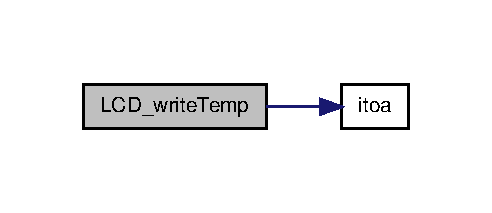
\includegraphics[width=236pt]{_l_c_d_8c_a34bb56ab53c7d9c0e363e59c48f5a959_cgraph}
\end{center}
\end{figure}




Here is the caller graph for this function\-:
\nopagebreak
\begin{figure}[H]
\begin{center}
\leavevmode
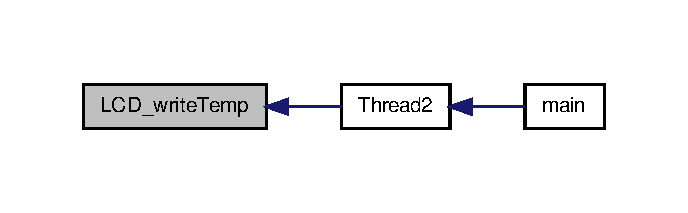
\includegraphics[width=330pt]{_l_c_d_8c_a34bb56ab53c7d9c0e363e59c48f5a959_icgraph}
\end{center}
\end{figure}


\index{L\-C\-D.\-c@{L\-C\-D.\-c}!L\-C\-D\-\_\-write\-Time@{L\-C\-D\-\_\-write\-Time}}
\index{L\-C\-D\-\_\-write\-Time@{L\-C\-D\-\_\-write\-Time}!LCD.c@{L\-C\-D.\-c}}
\subsubsection[{L\-C\-D\-\_\-write\-Time}]{\setlength{\rightskip}{0pt plus 5cm}void L\-C\-D\-\_\-write\-Time (
\begin{DoxyParamCaption}
\item[{R\-T\-C\-\_\-time\-\_\-t}]{time\-To\-Write}
\end{DoxyParamCaption}
)}\label{_l_c_d_8c_a86e9fbcb9579b78118f6add9d1e78ba8}


Idő megjelenítése a kijelzőn. 


\begin{DoxyParams}[1]{Paraméterek}
\mbox{\tt in}  & {\em time\-To\-Write} & Idő érték. \\
\hline
\end{DoxyParams}


Definíció a(z) L\-C\-D.\-c fájl 277. sorában.



A függvény hívási gráfja\-:\nopagebreak
\begin{figure}[H]
\begin{center}
\leavevmode
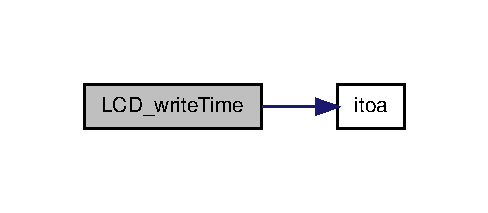
\includegraphics[width=234pt]{_l_c_d_8c_a86e9fbcb9579b78118f6add9d1e78ba8_cgraph}
\end{center}
\end{figure}




Here is the caller graph for this function\-:
\nopagebreak
\begin{figure}[H]
\begin{center}
\leavevmode
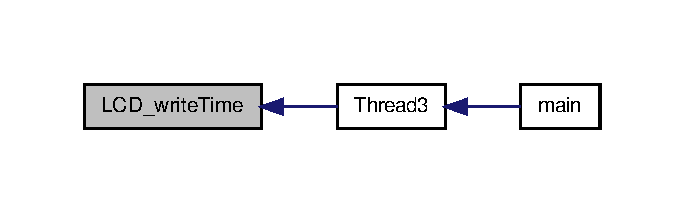
\includegraphics[width=328pt]{_l_c_d_8c_a86e9fbcb9579b78118f6add9d1e78ba8_icgraph}
\end{center}
\end{figure}


\index{L\-C\-D.\-c@{L\-C\-D.\-c}!L\-C\-D\-\_\-write\-U\-S\-B@{L\-C\-D\-\_\-write\-U\-S\-B}}
\index{L\-C\-D\-\_\-write\-U\-S\-B@{L\-C\-D\-\_\-write\-U\-S\-B}!LCD.c@{L\-C\-D.\-c}}
\subsubsection[{L\-C\-D\-\_\-write\-U\-S\-B}]{\setlength{\rightskip}{0pt plus 5cm}void L\-C\-D\-\_\-write\-U\-S\-B (
\begin{DoxyParamCaption}
{}
\end{DoxyParamCaption}
)}\label{_l_c_d_8c_ab128f02215b4c1e80793338995eada18}


U\-S\-B felirat megjelenítése a kijelzőn. 



Definíció a(z) L\-C\-D.\-c fájl 302. sorában.



Here is the caller graph for this function\-:
\nopagebreak
\begin{figure}[H]
\begin{center}
\leavevmode
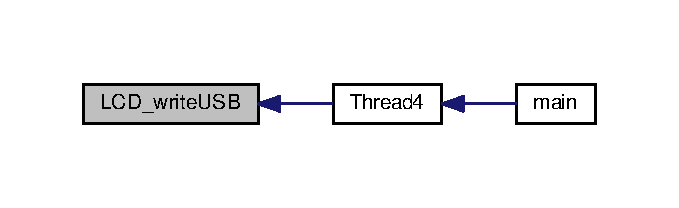
\includegraphics[width=326pt]{_l_c_d_8c_ab128f02215b4c1e80793338995eada18_icgraph}
\end{center}
\end{figure}


\index{L\-C\-D.\-c@{L\-C\-D.\-c}!L\-C\-D\-\_\-write\-U\-S\-B\-\_\-delete@{L\-C\-D\-\_\-write\-U\-S\-B\-\_\-delete}}
\index{L\-C\-D\-\_\-write\-U\-S\-B\-\_\-delete@{L\-C\-D\-\_\-write\-U\-S\-B\-\_\-delete}!LCD.c@{L\-C\-D.\-c}}
\subsubsection[{L\-C\-D\-\_\-write\-U\-S\-B\-\_\-delete}]{\setlength{\rightskip}{0pt plus 5cm}void L\-C\-D\-\_\-write\-U\-S\-B\-\_\-delete (
\begin{DoxyParamCaption}
{}
\end{DoxyParamCaption}
)}\label{_l_c_d_8c_ad738a14f7ceaf0da125b1337a4e9e10b}


U\-S\-B felirat törlése a kijelzőről. 



Definíció a(z) L\-C\-D.\-c fájl 320. sorában.



Here is the caller graph for this function\-:
\nopagebreak
\begin{figure}[H]
\begin{center}
\leavevmode
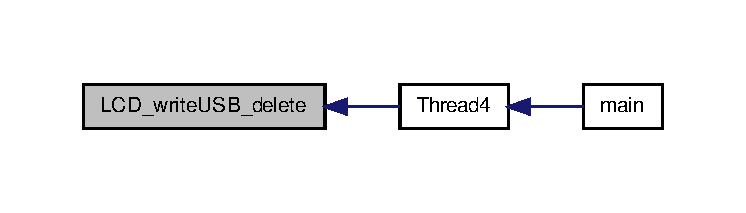
\includegraphics[width=350pt]{_l_c_d_8c_ad738a14f7ceaf0da125b1337a4e9e10b_icgraph}
\end{center}
\end{figure}



\section{/\-H\-D\-D/\-G\-I\-T/variometer/\-Altimeter/src/logger.c fájlreferencia}
\label{logger_8c}\index{/\-H\-D\-D/\-G\-I\-T/variometer/\-Altimeter/src/logger.\-c@{/\-H\-D\-D/\-G\-I\-T/variometer/\-Altimeter/src/logger.\-c}}
{\ttfamily \#include \char`\"{}logger.\-h\char`\"{}}\\*
{\ttfamily \#include \char`\"{}eeprom.\-h\char`\"{}}\\*
A logger.\-c definíciós fájl függési gráfja\-:
\nopagebreak
\begin{figure}[H]
\begin{center}
\leavevmode
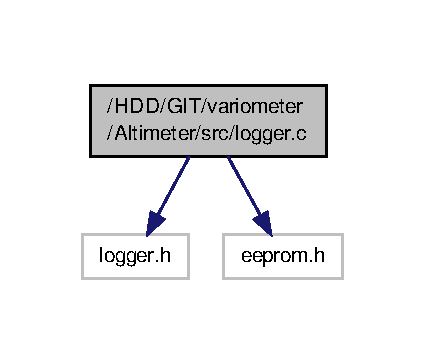
\includegraphics[width=204pt]{logger_8c__incl}
\end{center}
\end{figure}
\subsection*{Függvények}
\begin{DoxyCompactItemize}
\item 
void {\bf logger\-\_\-init} ()
\begin{DoxyCompactList}\small\item\em A naplózó alrendszer inicializálása. \end{DoxyCompactList}\item 
int {\bf logger\-\_\-log\-This} (log\-\_\-rec\-\_\-t $\ast$rec\-\_\-to\-\_\-log)
\begin{DoxyCompactList}\small\item\em A paraméterként kapott rekordot berakja a ringbufferbe, ahonnan később ki fog íródni az E\-E\-P\-R\-O\-M-\/ba. \end{DoxyCompactList}\item 
int {\bf logger\-\_\-write\-To\-E\-E} ()
\begin{DoxyCompactList}\small\item\em A ringbufferből kiír egy rekordot az E\-E\-P\-R\-O\-M-\/ba. \end{DoxyCompactList}\item 
uint16\-\_\-t {\bf logger\-\_\-read\-From\-E\-E} (log\-\_\-rec\-\_\-t $\ast$buffer, uint16\-\_\-t size\-\_\-in\-\_\-rec)
\begin{DoxyCompactList}\small\item\em Adott számú rekord kikérése az E\-E\-P\-R\-O\-M-\/ból. \end{DoxyCompactList}\item 
int {\bf logger\-\_\-delete\-Log} ()
\begin{DoxyCompactList}\small\item\em Kitörli a naplóállományt az E\-E\-P\-R\-O\-M-\/ból. \end{DoxyCompactList}\end{DoxyCompactItemize}


\subsection{Függvények dokumentációja}
\index{logger.\-c@{logger.\-c}!logger\-\_\-delete\-Log@{logger\-\_\-delete\-Log}}
\index{logger\-\_\-delete\-Log@{logger\-\_\-delete\-Log}!logger.c@{logger.\-c}}
\subsubsection[{logger\-\_\-delete\-Log}]{\setlength{\rightskip}{0pt plus 5cm}int logger\-\_\-delete\-Log (
\begin{DoxyParamCaption}
{}
\end{DoxyParamCaption}
)}\label{logger_8c_a14c8fca7ded47975eb3ca731a8eacfef}


Kitörli a naplóállományt az E\-E\-P\-R\-O\-M-\/ból. 

(Még nincs implementálva.) \begin{DoxyReturn}{Visszatérési érték}
0. 
\end{DoxyReturn}


Definíció a(z) logger.\-c fájl 107. sorában.

\index{logger.\-c@{logger.\-c}!logger\-\_\-init@{logger\-\_\-init}}
\index{logger\-\_\-init@{logger\-\_\-init}!logger.c@{logger.\-c}}
\subsubsection[{logger\-\_\-init}]{\setlength{\rightskip}{0pt plus 5cm}void logger\-\_\-init (
\begin{DoxyParamCaption}
{}
\end{DoxyParamCaption}
)}\label{logger_8c_acca02da5a5a8b842893ecc30ea12fda7}


A naplózó alrendszer inicializálása. 



Definíció a(z) logger.\-c fájl 18. sorában.



A függvény hívási gráfja\-:
\nopagebreak
\begin{figure}[H]
\begin{center}
\leavevmode
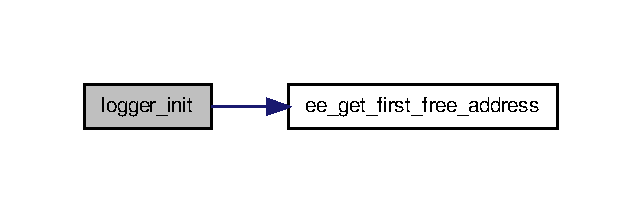
\includegraphics[width=308pt]{logger_8c_acca02da5a5a8b842893ecc30ea12fda7_cgraph}
\end{center}
\end{figure}




Here is the caller graph for this function\-:
\nopagebreak
\begin{figure}[H]
\begin{center}
\leavevmode
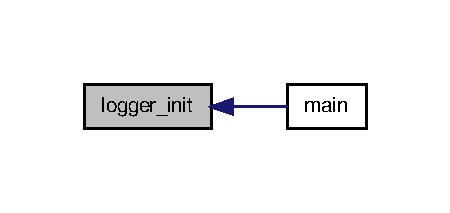
\includegraphics[width=216pt]{logger_8c_acca02da5a5a8b842893ecc30ea12fda7_icgraph}
\end{center}
\end{figure}


\index{logger.\-c@{logger.\-c}!logger\-\_\-log\-This@{logger\-\_\-log\-This}}
\index{logger\-\_\-log\-This@{logger\-\_\-log\-This}!logger.c@{logger.\-c}}
\subsubsection[{logger\-\_\-log\-This}]{\setlength{\rightskip}{0pt plus 5cm}int logger\-\_\-log\-This (
\begin{DoxyParamCaption}
\item[{log\-\_\-rec\-\_\-t $\ast$}]{rec\-\_\-to\-\_\-log}
\end{DoxyParamCaption}
)}\label{logger_8c_ab32b0e36c611a22cba880cc3aacda3db}


A paraméterként kapott rekordot berakja a ringbufferbe, ahonnan később ki fog íródni az E\-E\-P\-R\-O\-M-\/ba. 


\begin{DoxyParams}[1]{Paraméterek}
\mbox{\tt in}  & {\em rec\-\_\-to\-\_\-log} & A naplózandó rekord. \\
\hline
\end{DoxyParams}
\begin{DoxyReturn}{Visszatérési érték}
0 -\/ normál működés, 1 -\/ túlcsordulás, a legrégebbi elem felülíródott. 
\end{DoxyReturn}


Definíció a(z) logger.\-c fájl 37. sorában.



Here is the caller graph for this function\-:
\nopagebreak
\begin{figure}[H]
\begin{center}
\leavevmode
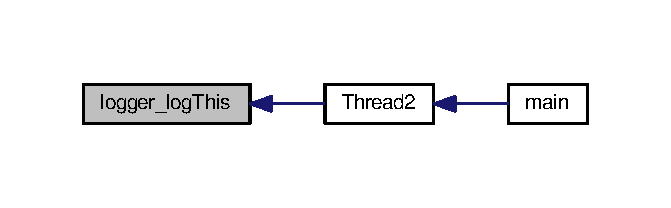
\includegraphics[width=322pt]{logger_8c_ab32b0e36c611a22cba880cc3aacda3db_icgraph}
\end{center}
\end{figure}


\index{logger.\-c@{logger.\-c}!logger\-\_\-read\-From\-E\-E@{logger\-\_\-read\-From\-E\-E}}
\index{logger\-\_\-read\-From\-E\-E@{logger\-\_\-read\-From\-E\-E}!logger.c@{logger.\-c}}
\subsubsection[{logger\-\_\-read\-From\-E\-E}]{\setlength{\rightskip}{0pt plus 5cm}uint16\-\_\-t logger\-\_\-read\-From\-E\-E (
\begin{DoxyParamCaption}
\item[{log\-\_\-rec\-\_\-t $\ast$}]{buffer, }
\item[{uint16\-\_\-t}]{size\-\_\-in\-\_\-rec}
\end{DoxyParamCaption}
)}\label{logger_8c_a6d5881c4551c02ba1ca81719d375eeac}


Adott számú rekord kikérése az E\-E\-P\-R\-O\-M-\/ból. 


\begin{DoxyParams}[1]{Paraméterek}
\mbox{\tt out}  & {\em buffer} & Mutató az eredménybufferre. \\
\hline
\mbox{\tt in}  & {\em size\-\_\-in\-\_\-rec} & Rekordok száma. \\
\hline
\end{DoxyParams}
\begin{DoxyReturn}{Visszatérési érték}
A következő kiolvasható rekord címe. 
\end{DoxyReturn}


Definíció a(z) logger.\-c fájl 96. sorában.



A függvény hívási gráfja\-:
\nopagebreak
\begin{figure}[H]
\begin{center}
\leavevmode
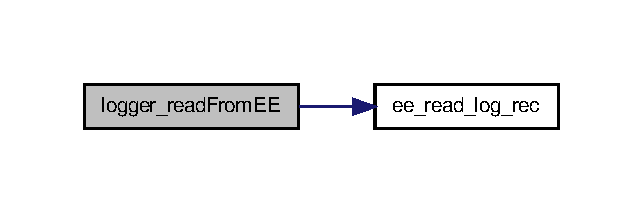
\includegraphics[width=308pt]{logger_8c_a6d5881c4551c02ba1ca81719d375eeac_cgraph}
\end{center}
\end{figure}


\index{logger.\-c@{logger.\-c}!logger\-\_\-write\-To\-E\-E@{logger\-\_\-write\-To\-E\-E}}
\index{logger\-\_\-write\-To\-E\-E@{logger\-\_\-write\-To\-E\-E}!logger.c@{logger.\-c}}
\subsubsection[{logger\-\_\-write\-To\-E\-E}]{\setlength{\rightskip}{0pt plus 5cm}int logger\-\_\-write\-To\-E\-E (
\begin{DoxyParamCaption}
{}
\end{DoxyParamCaption}
)}\label{logger_8c_a8f9e5decfda36c73889dcb1ebd212022}


A ringbufferből kiír egy rekordot az E\-E\-P\-R\-O\-M-\/ba. 

Ha az írás sikeres volt, törli az elemet a bufferből. \begin{DoxyReturn}{Visszatérési érték}
A ringbufferben maradt elemek száma. 
\end{DoxyReturn}


Definíció a(z) logger.\-c fájl 69. sorában.



A függvény hívási gráfja\-:
\nopagebreak
\begin{figure}[H]
\begin{center}
\leavevmode
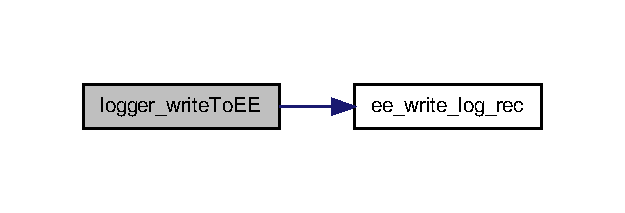
\includegraphics[width=300pt]{logger_8c_a8f9e5decfda36c73889dcb1ebd212022_cgraph}
\end{center}
\end{figure}




Here is the caller graph for this function\-:
\nopagebreak
\begin{figure}[H]
\begin{center}
\leavevmode
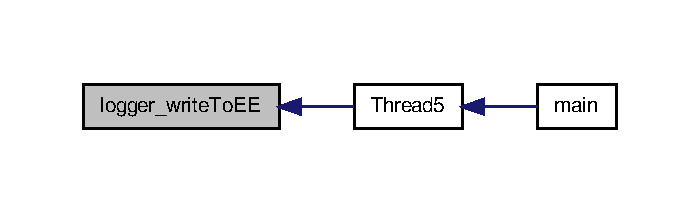
\includegraphics[width=336pt]{logger_8c_a8f9e5decfda36c73889dcb1ebd212022_icgraph}
\end{center}
\end{figure}



\section{src/main.c fájlreferencia}
\label{main_8c}\index{src/main.\-c@{src/main.\-c}}
{\ttfamily \#include \char`\"{}ch.\-h\char`\"{}}\\*
{\ttfamily \#include \char`\"{}hal.\-h\char`\"{}}\\*
{\ttfamily \#include \char`\"{}L\-C\-D.\-h\char`\"{}}\\*
{\ttfamily \#include \char`\"{}H\-P03.\-h\char`\"{}}\\*
{\ttfamily \#include \char`\"{}R\-T\-C\-\_\-r2051.\-h\char`\"{}}\\*
{\ttfamily \#include \char`\"{}Virtual\-Serial.\-h\char`\"{}}\\*
{\ttfamily \#include \char`\"{}Kalman.\-h\char`\"{}}\\*
{\ttfamily \#include \char`\"{}logger.\-h\char`\"{}}\\*
{\ttfamily \#include \char`\"{}periph.\-h\char`\"{}}\\*
{\ttfamily \#include \char`\"{}tasks.\-h\char`\"{}}\\*
A main.\-c definíciós fájl függési gráfja\-:
\nopagebreak
\begin{figure}[H]
\begin{center}
\leavevmode
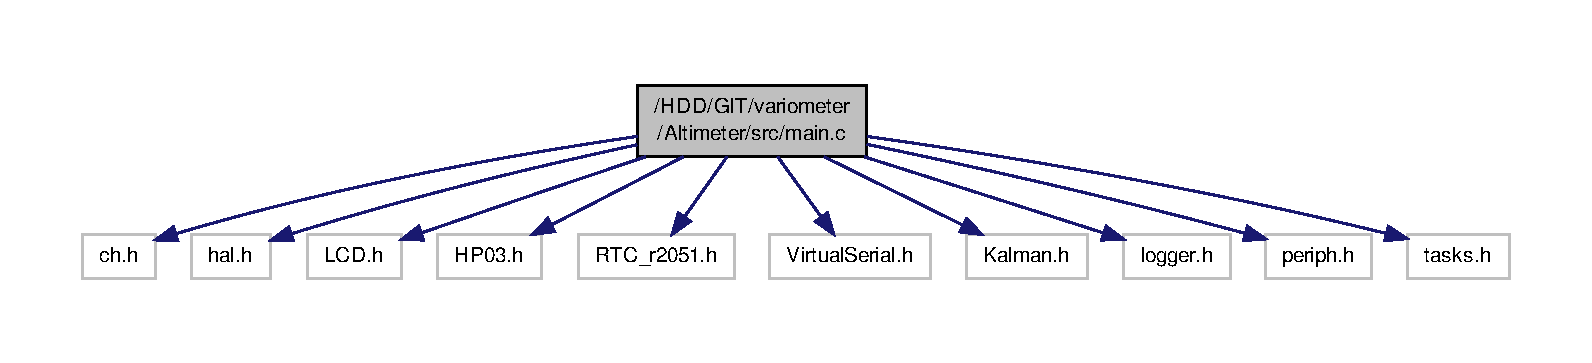
\includegraphics[width=350pt]{main_8c__incl}
\end{center}
\end{figure}
\subsection*{Függvények}
\begin{DoxyCompactItemize}
\item 
int {\bf main} (void)
\begin{DoxyCompactList}\small\item\em A szoftver belépési pontja. \end{DoxyCompactList}\end{DoxyCompactItemize}
\subsection*{Változók}
\begin{DoxyCompactItemize}
\item 
volatile R\-T\-C\-\_\-time\-\_\-t {\bf actual\-Time}
\item 
volatile R\-T\-C\-\_\-date\-\_\-t {\bf actual\-Date}
\item 
volatile float {\bf calculated\-Sea\-Level\-Pressure} = 0
\item 
Binary\-Semaphore {\bf bin\-Sem\-\_\-\-T5}
\item 
volatile bool\-\_\-t {\bf can\-T5\-Run} = F\-A\-L\-S\-E
\end{DoxyCompactItemize}


\subsection{Függvények dokumentációja}
\index{main.\-c@{main.\-c}!main@{main}}
\index{main@{main}!main.c@{main.\-c}}
\subsubsection[{main}]{\setlength{\rightskip}{0pt plus 5cm}int main (
\begin{DoxyParamCaption}
\item[{void}]{}
\end{DoxyParamCaption}
)}\label{main_8c_a840291bc02cba5474a4cb46a9b9566fe}


A szoftver belépési pontja. 

Rendszer-\/inicializálás.
\begin{DoxyItemize}
\item H\-A\-L inicializálás (So\-C és kártya specifikus)
\item Kernel inicializálás, a \doxyref{main()}{o.}{main_8c_a840291bc02cba5474a4cb46a9b9566fe} függvényből szál lesz és az R\-T\-O\-S elindul.
\end{DoxyItemize}

Az S\-P\-I és az I2\-C aktiválása.

A perifériák és modulok inicializálása.

A tengerszintre átszámított légnyomás kiszámíttatása. Az első kiolvasás a szenzorból nem biztos, hogy helyes, ezért két kiolvasás szükséges.

Aktuális dátum kiolvasása az R\-T\-C-\/ből.

Hangszóró tesztelése (P\-W\-M).

Háttérvilágítás bekapcsolása.

Szálak létrehozása.

Definíció a(z) main.\-c fájl 25. sorában.



A függvény hívási gráfja\-:
\nopagebreak
\begin{figure}[H]
\begin{center}
\leavevmode
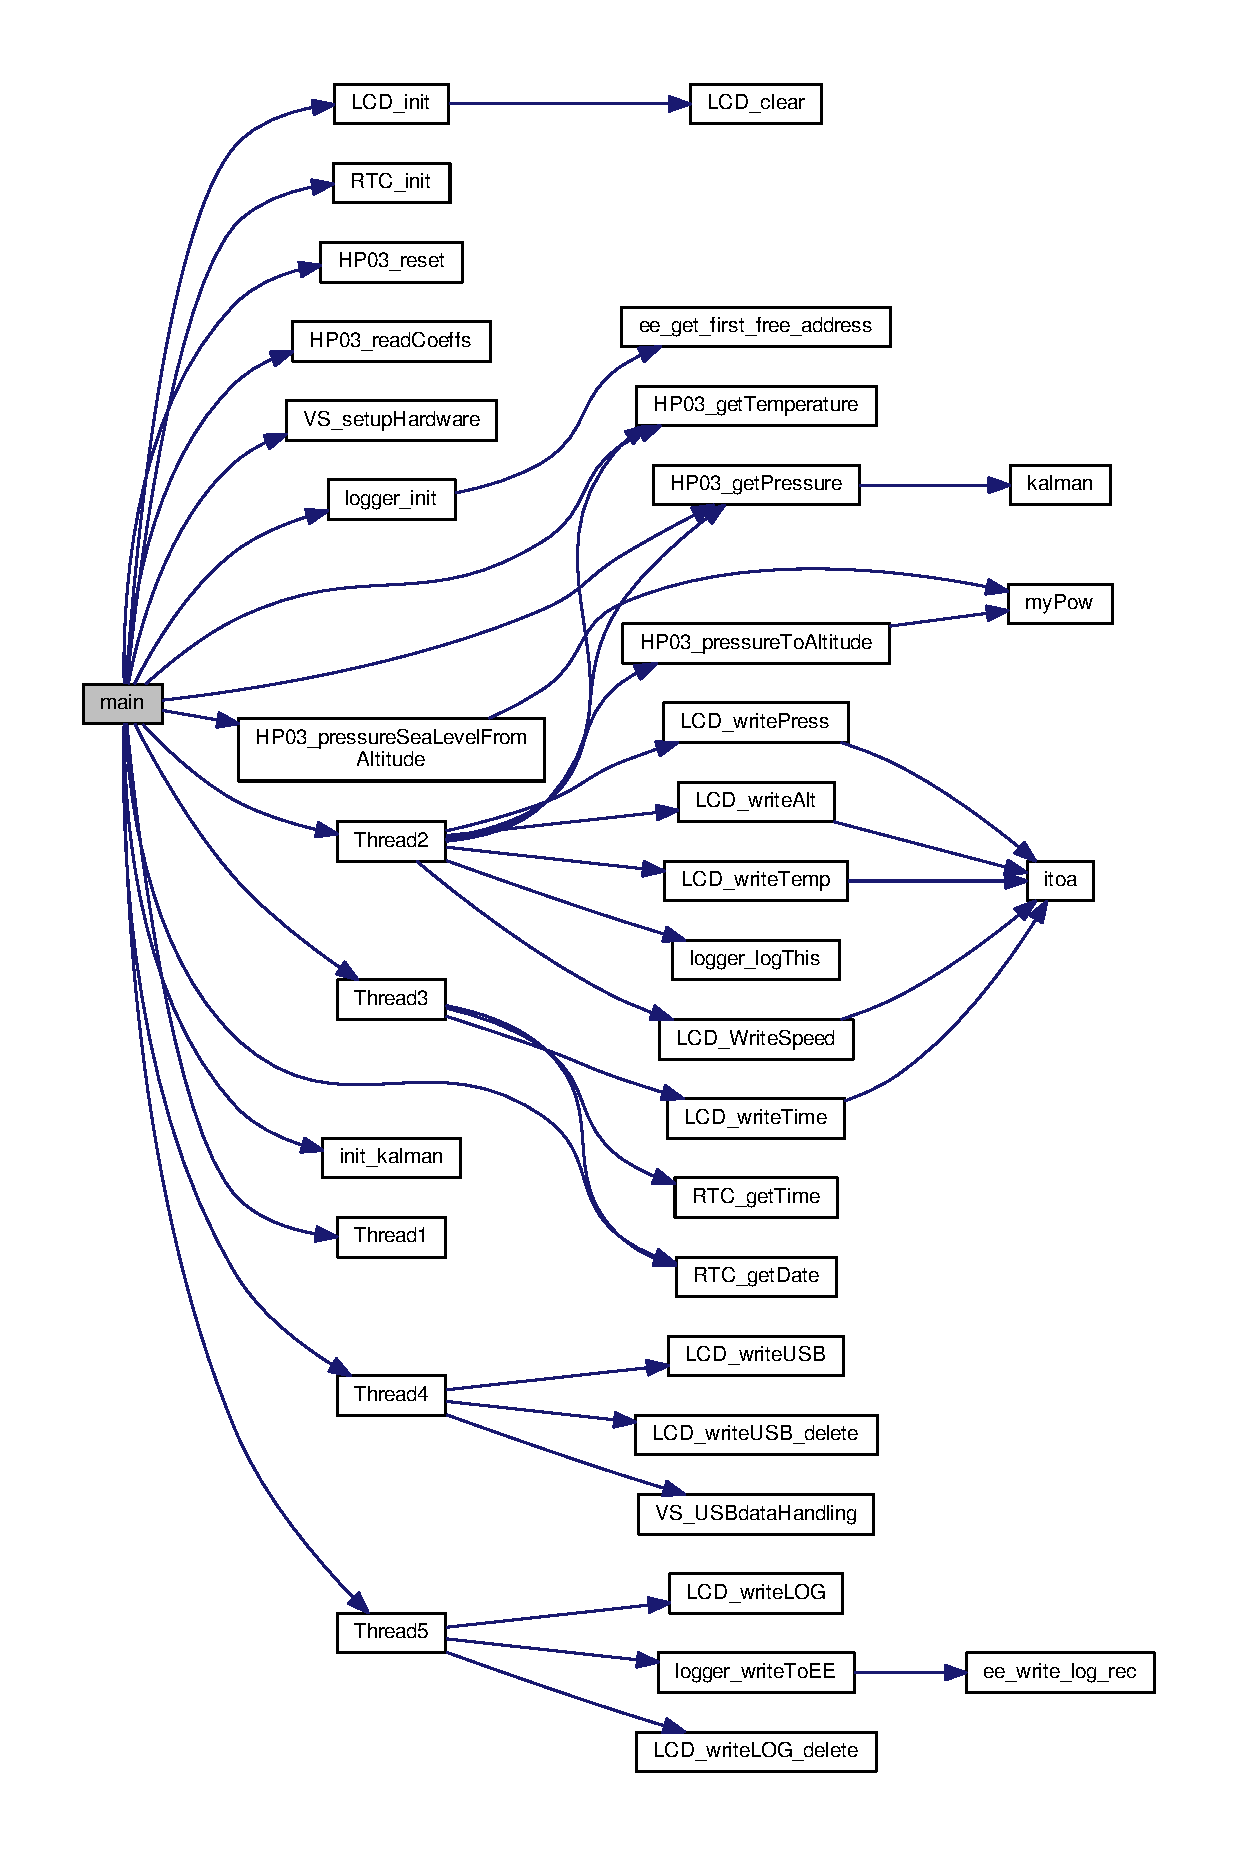
\includegraphics[width=350pt]{main_8c_a840291bc02cba5474a4cb46a9b9566fe_cgraph}
\end{center}
\end{figure}




\subsection{Változók dokumentációja}
\index{main.\-c@{main.\-c}!actual\-Date@{actual\-Date}}
\index{actual\-Date@{actual\-Date}!main.c@{main.\-c}}
\subsubsection[{actual\-Date}]{\setlength{\rightskip}{0pt plus 5cm}volatile R\-T\-C\-\_\-date\-\_\-t actual\-Date}\label{main_8c_a1fcf2a74e06883fb690c0c062bf9408c}


Definíció a(z) main.\-c fájl 17. sorában.

\index{main.\-c@{main.\-c}!actual\-Time@{actual\-Time}}
\index{actual\-Time@{actual\-Time}!main.c@{main.\-c}}
\subsubsection[{actual\-Time}]{\setlength{\rightskip}{0pt plus 5cm}volatile R\-T\-C\-\_\-time\-\_\-t actual\-Time}\label{main_8c_adf161c6b74a74517e1683aa5f3cc038a}


Definíció a(z) main.\-c fájl 16. sorában.

\index{main.\-c@{main.\-c}!bin\-Sem\-\_\-\-T5@{bin\-Sem\-\_\-\-T5}}
\index{bin\-Sem\-\_\-\-T5@{bin\-Sem\-\_\-\-T5}!main.c@{main.\-c}}
\subsubsection[{bin\-Sem\-\_\-\-T5}]{\setlength{\rightskip}{0pt plus 5cm}Binary\-Semaphore bin\-Sem\-\_\-\-T5}\label{main_8c_ae8441706b2e2119d6ab6c6ba48dfe7c3}


Definíció a(z) main.\-c fájl 19. sorában.

\index{main.\-c@{main.\-c}!calculated\-Sea\-Level\-Pressure@{calculated\-Sea\-Level\-Pressure}}
\index{calculated\-Sea\-Level\-Pressure@{calculated\-Sea\-Level\-Pressure}!main.c@{main.\-c}}
\subsubsection[{calculated\-Sea\-Level\-Pressure}]{\setlength{\rightskip}{0pt plus 5cm}volatile float calculated\-Sea\-Level\-Pressure = 0}\label{main_8c_ae33a247a27845609a2f5d2893060d2bb}


Definíció a(z) main.\-c fájl 18. sorában.

\index{main.\-c@{main.\-c}!can\-T5\-Run@{can\-T5\-Run}}
\index{can\-T5\-Run@{can\-T5\-Run}!main.c@{main.\-c}}
\subsubsection[{can\-T5\-Run}]{\setlength{\rightskip}{0pt plus 5cm}volatile bool\-\_\-t can\-T5\-Run = F\-A\-L\-S\-E}\label{main_8c_a6858a7f7f4872eaa5dcc054641626c55}


Definíció a(z) main.\-c fájl 20. sorában.


\section{src/mymath.c fájlreferencia}
\label{mymath_8c}\index{src/mymath.\-c@{src/mymath.\-c}}
{\ttfamily \#include \char`\"{}mymath.\-h\char`\"{}}\\*
A mymath.\-c definíciós fájl függési gráfja\-:
\nopagebreak
\begin{figure}[H]
\begin{center}
\leavevmode
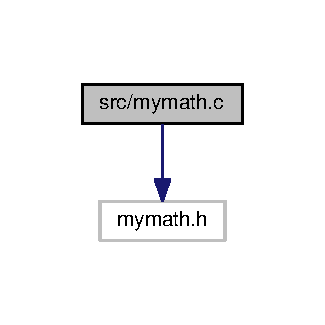
\includegraphics[width=156pt]{mymath_8c__incl}
\end{center}
\end{figure}
\subsection*{Függvények}
\begin{DoxyCompactItemize}
\item 
float {\bf my\-Pow} (float a, float b)
\end{DoxyCompactItemize}


\subsection{Függvények dokumentációja}
\index{mymath.\-c@{mymath.\-c}!my\-Pow@{my\-Pow}}
\index{my\-Pow@{my\-Pow}!mymath.c@{mymath.\-c}}
\subsubsection[{my\-Pow}]{\setlength{\rightskip}{0pt plus 5cm}float my\-Pow (
\begin{DoxyParamCaption}
\item[{float}]{a, }
\item[{float}]{b}
\end{DoxyParamCaption}
)}\label{mymath_8c_a73b3c2799ff1322f5f274157cbfdd4a1}


Definíció a(z) mymath.\-c fájl 70. sorában.



Here is the caller graph for this function\-:
\nopagebreak
\begin{figure}[H]
\begin{center}
\leavevmode
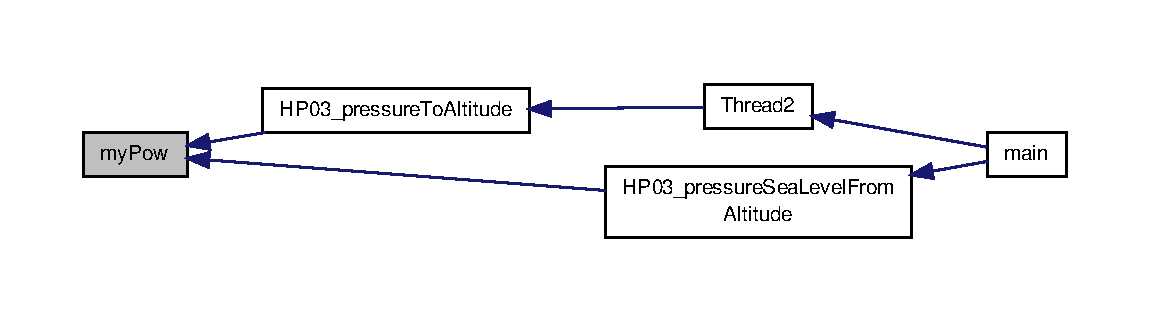
\includegraphics[width=350pt]{mymath_8c_a73b3c2799ff1322f5f274157cbfdd4a1_icgraph}
\end{center}
\end{figure}



\section{src/periph.c fájlreferencia}
\label{periph_8c}\index{src/periph.\-c@{src/periph.\-c}}
{\ttfamily \#include \char`\"{}ch.\-h\char`\"{}}\\*
{\ttfamily \#include \char`\"{}hal.\-h\char`\"{}}\\*
{\ttfamily \#include \char`\"{}periph.\-h\char`\"{}}\\*
A periph.\-c definíciós fájl függési gráfja\-:
\nopagebreak
\begin{figure}[H]
\begin{center}
\leavevmode
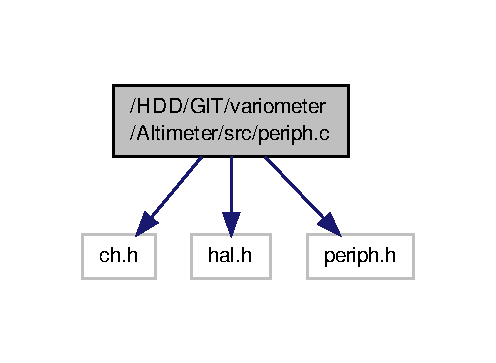
\includegraphics[width=240pt]{periph_8c__incl}
\end{center}
\end{figure}
\subsection*{Függvények}
\begin{DoxyCompactItemize}
\item 
void {\bf pwm3pcb} (P\-W\-M\-Driver $\ast$pwmp)
\begin{DoxyCompactList}\small\item\em Callback függvény. \end{DoxyCompactList}\item 
void {\bf pwm3c0cb} (P\-W\-M\-Driver $\ast$pwmp)
\end{DoxyCompactItemize}
\subsection*{Változók}
\begin{DoxyCompactItemize}
\item 
S\-P\-I\-Config {\bf spicfg}
\begin{DoxyCompactList}\small\item\em S\-P\-I konfiguráció (1\-M\-Hz, C\-P\-H\-A=0, C\-P\-O\-L=0). \end{DoxyCompactList}\item 
I2\-C\-Config {\bf i2ccfg}
\begin{DoxyCompactList}\small\item\em I2\-C konfiguráció (400k\-Hz). \end{DoxyCompactList}\item 
P\-W\-M\-Config {\bf pwmcfg}
\begin{DoxyCompactList}\small\item\em P\-W\-M konfiguráció. \end{DoxyCompactList}\end{DoxyCompactItemize}


\subsection{Függvények dokumentációja}
\index{periph.\-c@{periph.\-c}!pwm3c0cb@{pwm3c0cb}}
\index{pwm3c0cb@{pwm3c0cb}!periph.c@{periph.\-c}}
\subsubsection[{pwm3c0cb}]{\setlength{\rightskip}{0pt plus 5cm}void pwm3c0cb (
\begin{DoxyParamCaption}
\item[{P\-W\-M\-Driver $\ast$}]{pwmp}
\end{DoxyParamCaption}
)}\label{periph_8c_af6f3a2503083af2614563d0cc1f0c96c}


Definíció a(z) periph.\-c fájl 53. sorában.

\index{periph.\-c@{periph.\-c}!pwm3pcb@{pwm3pcb}}
\index{pwm3pcb@{pwm3pcb}!periph.c@{periph.\-c}}
\subsubsection[{pwm3pcb}]{\setlength{\rightskip}{0pt plus 5cm}void pwm3pcb (
\begin{DoxyParamCaption}
\item[{P\-W\-M\-Driver $\ast$}]{pwmp}
\end{DoxyParamCaption}
)}\label{periph_8c_ad3406d6a8fd6f21ccb106ecce466ec52}


Callback függvény. 



Definíció a(z) periph.\-c fájl 47. sorában.



\subsection{Változók dokumentációja}
\index{periph.\-c@{periph.\-c}!i2ccfg@{i2ccfg}}
\index{i2ccfg@{i2ccfg}!periph.c@{periph.\-c}}
\subsubsection[{i2ccfg}]{\setlength{\rightskip}{0pt plus 5cm}I2\-C\-Config i2ccfg}\label{periph_8c_a5dadd1387ac7b6a9a9bf2416cb1e2894}
{\bfseries Kezdő érték\-:}
\begin{DoxyCode}
= \{
    I2C\_FAST\_MODE\_PLUS,            
    48                             
\}
\end{DoxyCode}


I2\-C konfiguráció (400k\-Hz). 



Definíció a(z) periph.\-c fájl 26. sorában.

\index{periph.\-c@{periph.\-c}!pwmcfg@{pwmcfg}}
\index{pwmcfg@{pwmcfg}!periph.c@{periph.\-c}}
\subsubsection[{pwmcfg}]{\setlength{\rightskip}{0pt plus 5cm}P\-W\-M\-Config pwmcfg}\label{periph_8c_a902ad52cd507aae1615bd2858a47020d}
{\bfseries Kezdő érték\-:}
\begin{DoxyCode}
= \{
    100000,                          
       100,                          
    pwm3pcb,                         
    \{
        \{PWM\_OUTPUT\_ACTIVE\_LOW, pwm3c0cb\},
        \{PWM\_OUTPUT\_ACTIVE\_LOW, NULL\}
    \}
\}
\end{DoxyCode}


P\-W\-M konfiguráció. 



Definíció a(z) periph.\-c fájl 34. sorában.

\index{periph.\-c@{periph.\-c}!spicfg@{spicfg}}
\index{spicfg@{spicfg}!periph.c@{periph.\-c}}
\subsubsection[{spicfg}]{\setlength{\rightskip}{0pt plus 5cm}S\-P\-I\-Config spicfg}\label{periph_8c_afc4986c4ff59c9cd490bd7fd437f7c1a}
{\bfseries Kezdő érték\-:}
\begin{DoxyCode}
= \{
  NULL,
  GPIO0,
  GPIO0\_LCD\_SEL, 
  CR0\_DSS8BIT | CR0\_FRFSPI | CR0\_CLOCKRATE(0),
  48
\}
\end{DoxyCode}


S\-P\-I konfiguráció (1\-M\-Hz, C\-P\-H\-A=0, C\-P\-O\-L=0). 



Definíció a(z) periph.\-c fájl 15. sorában.


\section{src/\-R\-T\-C\-\_\-r2051.c fájlreferencia}
\label{_r_t_c__r2051_8c}\index{src/\-R\-T\-C\-\_\-r2051.\-c@{src/\-R\-T\-C\-\_\-r2051.\-c}}
{\ttfamily \#include \char`\"{}ch.\-h\char`\"{}}\\*
{\ttfamily \#include \char`\"{}hal.\-h\char`\"{}}\\*
{\ttfamily \#include \char`\"{}globals.\-h\char`\"{}}\\*
{\ttfamily \#include \char`\"{}R\-T\-C\-\_\-r2051.\-h\char`\"{}}\\*
A R\-T\-C\-\_\-r2051.\-c definíciós fájl függési gráfja\-:
\nopagebreak
\begin{figure}[H]
\begin{center}
\leavevmode
\includegraphics[width=337pt]{_r_t_c__r2051_8c__incl}
\end{center}
\end{figure}
\subsection*{Függvények}
\begin{DoxyCompactItemize}
\item 
void {\bf R\-T\-C\-\_\-init} ()
\begin{DoxyCompactList}\small\item\em A Real Time Clock áramkör inicializálása. \end{DoxyCompactList}\item 
void {\bf R\-T\-C\-\_\-set\-Time} (R\-T\-C\-\_\-time\-\_\-t time\-To\-Be\-Set)
\begin{DoxyCompactList}\small\item\em Beállítja az időt az R\-T\-C áramkörben. \end{DoxyCompactList}\item 
void {\bf R\-T\-C\-\_\-set\-Date} (R\-T\-C\-\_\-date\-\_\-t date\-To\-Be\-Set)
\begin{DoxyCompactList}\small\item\em Beállítja a dátumot az R\-T\-C áramkörben. \end{DoxyCompactList}\item 
R\-T\-C\-\_\-time\-\_\-t {\bf R\-T\-C\-\_\-get\-Time} ()
\begin{DoxyCompactList}\small\item\em Az idő kiolvasása az R\-T\-C áramkörből. \end{DoxyCompactList}\item 
R\-T\-C\-\_\-date\-\_\-t {\bf R\-T\-C\-\_\-get\-Date} ()
\begin{DoxyCompactList}\small\item\em A dátum kiolvasása az R\-T\-C áramkörből. \end{DoxyCompactList}\end{DoxyCompactItemize}


\subsection{Függvények dokumentációja}
\index{R\-T\-C\-\_\-r2051.\-c@{R\-T\-C\-\_\-r2051.\-c}!R\-T\-C\-\_\-get\-Date@{R\-T\-C\-\_\-get\-Date}}
\index{R\-T\-C\-\_\-get\-Date@{R\-T\-C\-\_\-get\-Date}!RTC_r2051.c@{R\-T\-C\-\_\-r2051.\-c}}
\subsubsection[{R\-T\-C\-\_\-get\-Date}]{\setlength{\rightskip}{0pt plus 5cm}R\-T\-C\-\_\-date\-\_\-t R\-T\-C\-\_\-get\-Date (
\begin{DoxyParamCaption}
{}
\end{DoxyParamCaption}
)}\label{_r_t_c__r2051_8c_abbeadb69d76ca80037803e6ecb3c74dc}


A dátum kiolvasása az R\-T\-C áramkörből. 

\begin{DoxyReturn}{Visszatérési érték}
Az aktuális dátum. 
\end{DoxyReturn}


Definíció a(z) R\-T\-C\-\_\-r2051.\-c fájl 141. sorában.



Here is the caller graph for this function\-:
\nopagebreak
\begin{figure}[H]
\begin{center}
\leavevmode
\includegraphics[width=320pt]{_r_t_c__r2051_8c_abbeadb69d76ca80037803e6ecb3c74dc_icgraph}
\end{center}
\end{figure}


\index{R\-T\-C\-\_\-r2051.\-c@{R\-T\-C\-\_\-r2051.\-c}!R\-T\-C\-\_\-get\-Time@{R\-T\-C\-\_\-get\-Time}}
\index{R\-T\-C\-\_\-get\-Time@{R\-T\-C\-\_\-get\-Time}!RTC_r2051.c@{R\-T\-C\-\_\-r2051.\-c}}
\subsubsection[{R\-T\-C\-\_\-get\-Time}]{\setlength{\rightskip}{0pt plus 5cm}R\-T\-C\-\_\-time\-\_\-t R\-T\-C\-\_\-get\-Time (
\begin{DoxyParamCaption}
{}
\end{DoxyParamCaption}
)}\label{_r_t_c__r2051_8c_a6e44f6b1a18d3d5b22189a130c3cdb81}


Az idő kiolvasása az R\-T\-C áramkörből. 

\begin{DoxyReturn}{Visszatérési érték}
Az aktuális idő. 
\end{DoxyReturn}


Definíció a(z) R\-T\-C\-\_\-r2051.\-c fájl 103. sorában.



Here is the caller graph for this function\-:
\nopagebreak
\begin{figure}[H]
\begin{center}
\leavevmode
\includegraphics[width=320pt]{_r_t_c__r2051_8c_a6e44f6b1a18d3d5b22189a130c3cdb81_icgraph}
\end{center}
\end{figure}


\index{R\-T\-C\-\_\-r2051.\-c@{R\-T\-C\-\_\-r2051.\-c}!R\-T\-C\-\_\-init@{R\-T\-C\-\_\-init}}
\index{R\-T\-C\-\_\-init@{R\-T\-C\-\_\-init}!RTC_r2051.c@{R\-T\-C\-\_\-r2051.\-c}}
\subsubsection[{R\-T\-C\-\_\-init}]{\setlength{\rightskip}{0pt plus 5cm}void R\-T\-C\-\_\-init (
\begin{DoxyParamCaption}
{}
\end{DoxyParamCaption}
)}\label{_r_t_c__r2051_8c_afd522e1615ce58a62a9e5592d420aed2}


A Real Time Clock áramkör inicializálása. 



Definíció a(z) R\-T\-C\-\_\-r2051.\-c fájl 17. sorában.



Here is the caller graph for this function\-:
\nopagebreak
\begin{figure}[H]
\begin{center}
\leavevmode
\includegraphics[width=210pt]{_r_t_c__r2051_8c_afd522e1615ce58a62a9e5592d420aed2_icgraph}
\end{center}
\end{figure}


\index{R\-T\-C\-\_\-r2051.\-c@{R\-T\-C\-\_\-r2051.\-c}!R\-T\-C\-\_\-set\-Date@{R\-T\-C\-\_\-set\-Date}}
\index{R\-T\-C\-\_\-set\-Date@{R\-T\-C\-\_\-set\-Date}!RTC_r2051.c@{R\-T\-C\-\_\-r2051.\-c}}
\subsubsection[{R\-T\-C\-\_\-set\-Date}]{\setlength{\rightskip}{0pt plus 5cm}void R\-T\-C\-\_\-set\-Date (
\begin{DoxyParamCaption}
\item[{R\-T\-C\-\_\-date\-\_\-t}]{date\-To\-Be\-Set}
\end{DoxyParamCaption}
)}\label{_r_t_c__r2051_8c_ac6e5230f6da5333c2aaa3620648b0c22}


Beállítja a dátumot az R\-T\-C áramkörben. 


\begin{DoxyParams}[1]{Paraméterek}
\mbox{\tt in}  & {\em date\-To\-Be\-Set} & A beállítandó dátum. \\
\hline
\end{DoxyParams}


Definíció a(z) R\-T\-C\-\_\-r2051.\-c fájl 75. sorában.

\index{R\-T\-C\-\_\-r2051.\-c@{R\-T\-C\-\_\-r2051.\-c}!R\-T\-C\-\_\-set\-Time@{R\-T\-C\-\_\-set\-Time}}
\index{R\-T\-C\-\_\-set\-Time@{R\-T\-C\-\_\-set\-Time}!RTC_r2051.c@{R\-T\-C\-\_\-r2051.\-c}}
\subsubsection[{R\-T\-C\-\_\-set\-Time}]{\setlength{\rightskip}{0pt plus 5cm}void R\-T\-C\-\_\-set\-Time (
\begin{DoxyParamCaption}
\item[{R\-T\-C\-\_\-time\-\_\-t}]{time\-To\-Be\-Set}
\end{DoxyParamCaption}
)}\label{_r_t_c__r2051_8c_acfa71727df5a732c5381776accb6eac3}


Beállítja az időt az R\-T\-C áramkörben. 


\begin{DoxyParams}[1]{Paraméterek}
\mbox{\tt in}  & {\em time\-To\-Be\-Set} & A beállítandó idő. \\
\hline
\end{DoxyParams}


Definíció a(z) R\-T\-C\-\_\-r2051.\-c fájl 49. sorában.


\section{src/tasks.c fájlreferencia}
\label{tasks_8c}\index{src/tasks.\-c@{src/tasks.\-c}}
{\ttfamily \#include \char`\"{}ch.\-h\char`\"{}}\\*
{\ttfamily \#include \char`\"{}hal.\-h\char`\"{}}\\*
{\ttfamily \#include \char`\"{}L\-C\-D.\-h\char`\"{}}\\*
{\ttfamily \#include \char`\"{}H\-P03.\-h\char`\"{}}\\*
{\ttfamily \#include \char`\"{}R\-T\-C\-\_\-r2051.\-h\char`\"{}}\\*
{\ttfamily \#include \char`\"{}Virtual\-Serial.\-h\char`\"{}}\\*
{\ttfamily \#include \char`\"{}logger.\-h\char`\"{}}\\*
{\ttfamily \#include \char`\"{}periph.\-h\char`\"{}}\\*
A tasks.\-c definíciós fájl függési gráfja\-:
\nopagebreak
\begin{figure}[H]
\begin{center}
\leavevmode
\includegraphics[width=350pt]{tasks_8c__incl}
\end{center}
\end{figure}
\subsection*{Függvények}
\begin{DoxyCompactItemize}
\item 
msg\-\_\-t {\bf Thread1} (void $\ast$arg)
\begin{DoxyCompactList}\small\item\em \char`\"{}\-Heart\-Beat\char`\"{} L\-E\-D villogtató szál. \end{DoxyCompactList}\item 
msg\-\_\-t {\bf Thread2} (void $\ast$arg)
\begin{DoxyCompactList}\small\item\em Nyomás és hőmérséklet kiolvasó szál. \end{DoxyCompactList}\item 
msg\-\_\-t {\bf Thread3} (void $\ast$arg)
\begin{DoxyCompactList}\small\item\em Dátum és idő kezelő szál. \end{DoxyCompactList}\item 
msg\-\_\-t {\bf Thread4} (void $\ast$arg)
\begin{DoxyCompactList}\small\item\em U\-S\-B kezelő szál. \end{DoxyCompactList}\item 
msg\-\_\-t {\bf Thread5} (void $\ast$arg)
\begin{DoxyCompactList}\small\item\em E\-E\-P\-R\-O\-M író szál (ringbuffer -\/$>$ E\-E\-P\-R\-O\-M). \end{DoxyCompactList}\end{DoxyCompactItemize}
\subsection*{Változók}
\begin{DoxyCompactItemize}
\item 
volatile R\-T\-C\-\_\-time\-\_\-t {\bf actual\-Time}
\item 
volatile R\-T\-C\-\_\-date\-\_\-t {\bf actual\-Date}
\item 
volatile float {\bf calculated\-Sea\-Level\-Pressure}
\item 
Binary\-Semaphore {\bf bin\-Sem\-\_\-\-T5}
\item 
bool\-\_\-t {\bf can\-T5\-Run}
\item 
U\-S\-B\-\_\-\-Class\-Info\-\_\-\-C\-D\-C\-\_\-\-Device\-\_\-t {\bf Virtual\-Serial\-\_\-\-C\-D\-C\-\_\-\-Interface}
\begin{DoxyCompactList}\small\item\em L\-P\-C\-U\-S\-Blib C\-D\-C Class driver interfész konfiguráció és állapot-\/információ. \end{DoxyCompactList}\end{DoxyCompactItemize}


\subsection{Függvények dokumentációja}
\index{tasks.\-c@{tasks.\-c}!Thread1@{Thread1}}
\index{Thread1@{Thread1}!tasks.c@{tasks.\-c}}
\subsubsection[{Thread1}]{\setlength{\rightskip}{0pt plus 5cm}msg\-\_\-t Thread1 (
\begin{DoxyParamCaption}
\item[{void $\ast$}]{arg}
\end{DoxyParamCaption}
)}\label{tasks_8c_a0af304e6c5bca609f1da9a35a49da5c6}


\char`\"{}\-Heart\-Beat\char`\"{} L\-E\-D villogtató szál. 



Definíció a(z) tasks.\-c fájl 27. sorában.



Here is the caller graph for this function\-:
\nopagebreak
\begin{figure}[H]
\begin{center}
\leavevmode
\includegraphics[width=206pt]{tasks_8c_a0af304e6c5bca609f1da9a35a49da5c6_icgraph}
\end{center}
\end{figure}


\index{tasks.\-c@{tasks.\-c}!Thread2@{Thread2}}
\index{Thread2@{Thread2}!tasks.c@{tasks.\-c}}
\subsubsection[{Thread2}]{\setlength{\rightskip}{0pt plus 5cm}msg\-\_\-t Thread2 (
\begin{DoxyParamCaption}
\item[{void $\ast$}]{arg}
\end{DoxyParamCaption}
)}\label{tasks_8c_afc0a4f34ef3333216c2f7c0de2b1f9aa}


Nyomás és hőmérséklet kiolvasó szál. 



Definíció a(z) tasks.\-c fájl 44. sorában.



A függvény hívási gráfja\-:
\nopagebreak
\begin{figure}[H]
\begin{center}
\leavevmode
\includegraphics[width=350pt]{tasks_8c_afc0a4f34ef3333216c2f7c0de2b1f9aa_cgraph}
\end{center}
\end{figure}




Here is the caller graph for this function\-:
\nopagebreak
\begin{figure}[H]
\begin{center}
\leavevmode
\includegraphics[width=206pt]{tasks_8c_afc0a4f34ef3333216c2f7c0de2b1f9aa_icgraph}
\end{center}
\end{figure}


\index{tasks.\-c@{tasks.\-c}!Thread3@{Thread3}}
\index{Thread3@{Thread3}!tasks.c@{tasks.\-c}}
\subsubsection[{Thread3}]{\setlength{\rightskip}{0pt plus 5cm}msg\-\_\-t Thread3 (
\begin{DoxyParamCaption}
\item[{void $\ast$}]{arg}
\end{DoxyParamCaption}
)}\label{tasks_8c_a3287156dd96a38e39fa70850b4c6fa38}


Dátum és idő kezelő szál. 



Definíció a(z) tasks.\-c fájl 113. sorában.



A függvény hívási gráfja\-:\nopagebreak
\begin{figure}[H]
\begin{center}
\leavevmode
\includegraphics[width=322pt]{tasks_8c_a3287156dd96a38e39fa70850b4c6fa38_cgraph}
\end{center}
\end{figure}




Here is the caller graph for this function\-:
\nopagebreak
\begin{figure}[H]
\begin{center}
\leavevmode
\includegraphics[width=206pt]{tasks_8c_a3287156dd96a38e39fa70850b4c6fa38_icgraph}
\end{center}
\end{figure}


\index{tasks.\-c@{tasks.\-c}!Thread4@{Thread4}}
\index{Thread4@{Thread4}!tasks.c@{tasks.\-c}}
\subsubsection[{Thread4}]{\setlength{\rightskip}{0pt plus 5cm}msg\-\_\-t Thread4 (
\begin{DoxyParamCaption}
\item[{void $\ast$}]{arg}
\end{DoxyParamCaption}
)}\label{tasks_8c_ad2036d3514561ba8a748ff170baf1e3a}


U\-S\-B kezelő szál. 



Definíció a(z) tasks.\-c fájl 136. sorában.



A függvény hívási gráfja\-:
\nopagebreak
\begin{figure}[H]
\begin{center}
\leavevmode
\includegraphics[width=284pt]{tasks_8c_ad2036d3514561ba8a748ff170baf1e3a_cgraph}
\end{center}
\end{figure}




Here is the caller graph for this function\-:
\nopagebreak
\begin{figure}[H]
\begin{center}
\leavevmode
\includegraphics[width=206pt]{tasks_8c_ad2036d3514561ba8a748ff170baf1e3a_icgraph}
\end{center}
\end{figure}


\index{tasks.\-c@{tasks.\-c}!Thread5@{Thread5}}
\index{Thread5@{Thread5}!tasks.c@{tasks.\-c}}
\subsubsection[{Thread5}]{\setlength{\rightskip}{0pt plus 5cm}msg\-\_\-t Thread5 (
\begin{DoxyParamCaption}
\item[{void $\ast$}]{arg}
\end{DoxyParamCaption}
)}\label{tasks_8c_aad01c280ed05ea63627f5518167c5003}


E\-E\-P\-R\-O\-M író szál (ringbuffer -\/$>$ E\-E\-P\-R\-O\-M). 



Definíció a(z) tasks.\-c fájl 164. sorában.



A függvény hívási gráfja\-:
\nopagebreak
\begin{figure}[H]
\begin{center}
\leavevmode
\includegraphics[width=350pt]{tasks_8c_aad01c280ed05ea63627f5518167c5003_cgraph}
\end{center}
\end{figure}




Here is the caller graph for this function\-:
\nopagebreak
\begin{figure}[H]
\begin{center}
\leavevmode
\includegraphics[width=206pt]{tasks_8c_aad01c280ed05ea63627f5518167c5003_icgraph}
\end{center}
\end{figure}




\subsection{Változók dokumentációja}
\index{tasks.\-c@{tasks.\-c}!actual\-Date@{actual\-Date}}
\index{actual\-Date@{actual\-Date}!tasks.c@{tasks.\-c}}
\subsubsection[{actual\-Date}]{\setlength{\rightskip}{0pt plus 5cm}volatile R\-T\-C\-\_\-date\-\_\-t actual\-Date}\label{tasks_8c_a1fcf2a74e06883fb690c0c062bf9408c}


Definíció a(z) main.\-c fájl 17. sorában.

\index{tasks.\-c@{tasks.\-c}!actual\-Time@{actual\-Time}}
\index{actual\-Time@{actual\-Time}!tasks.c@{tasks.\-c}}
\subsubsection[{actual\-Time}]{\setlength{\rightskip}{0pt plus 5cm}volatile R\-T\-C\-\_\-time\-\_\-t actual\-Time}\label{tasks_8c_adf161c6b74a74517e1683aa5f3cc038a}


Definíció a(z) main.\-c fájl 16. sorában.

\index{tasks.\-c@{tasks.\-c}!bin\-Sem\-\_\-\-T5@{bin\-Sem\-\_\-\-T5}}
\index{bin\-Sem\-\_\-\-T5@{bin\-Sem\-\_\-\-T5}!tasks.c@{tasks.\-c}}
\subsubsection[{bin\-Sem\-\_\-\-T5}]{\setlength{\rightskip}{0pt plus 5cm}Binary\-Semaphore bin\-Sem\-\_\-\-T5}\label{tasks_8c_ae8441706b2e2119d6ab6c6ba48dfe7c3}


Definíció a(z) main.\-c fájl 19. sorában.

\index{tasks.\-c@{tasks.\-c}!calculated\-Sea\-Level\-Pressure@{calculated\-Sea\-Level\-Pressure}}
\index{calculated\-Sea\-Level\-Pressure@{calculated\-Sea\-Level\-Pressure}!tasks.c@{tasks.\-c}}
\subsubsection[{calculated\-Sea\-Level\-Pressure}]{\setlength{\rightskip}{0pt plus 5cm}volatile float calculated\-Sea\-Level\-Pressure}\label{tasks_8c_ae33a247a27845609a2f5d2893060d2bb}


Definíció a(z) main.\-c fájl 18. sorában.

\index{tasks.\-c@{tasks.\-c}!can\-T5\-Run@{can\-T5\-Run}}
\index{can\-T5\-Run@{can\-T5\-Run}!tasks.c@{tasks.\-c}}
\subsubsection[{can\-T5\-Run}]{\setlength{\rightskip}{0pt plus 5cm}bool\-\_\-t can\-T5\-Run}\label{tasks_8c_a128bc2ef2b7821fb43dc85d860ce6289}


Definíció a(z) main.\-c fájl 20. sorában.

\index{tasks.\-c@{tasks.\-c}!Virtual\-Serial\-\_\-\-C\-D\-C\-\_\-\-Interface@{Virtual\-Serial\-\_\-\-C\-D\-C\-\_\-\-Interface}}
\index{Virtual\-Serial\-\_\-\-C\-D\-C\-\_\-\-Interface@{Virtual\-Serial\-\_\-\-C\-D\-C\-\_\-\-Interface}!tasks.c@{tasks.\-c}}
\subsubsection[{Virtual\-Serial\-\_\-\-C\-D\-C\-\_\-\-Interface}]{\setlength{\rightskip}{0pt plus 5cm}U\-S\-B\-\_\-\-Class\-Info\-\_\-\-C\-D\-C\-\_\-\-Device\-\_\-t Virtual\-Serial\-\_\-\-C\-D\-C\-\_\-\-Interface}\label{tasks_8c_a6abff48bf476b7a0b5d81012d90058a6}


L\-P\-C\-U\-S\-Blib C\-D\-C Class driver interfész konfiguráció és állapot-\/információ. 

Ez a struktúra adódik át minden C\-D\-C Class driver függvénynek. 

Definíció a(z) Virtual\-Serial.\-c fájl 14. sorában.


\section{src/\-Virtual\-Serial.c fájlreferencia}
\label{_virtual_serial_8c}\index{src/\-Virtual\-Serial.\-c@{src/\-Virtual\-Serial.\-c}}
{\ttfamily \#include \char`\"{}Virtual\-Serial.\-h\char`\"{}}\\*
{\ttfamily \#include \char`\"{}ch.\-h\char`\"{}}\\*
{\ttfamily \#include \char`\"{}logger.\-h\char`\"{}}\\*
{\ttfamily \#include $<$string.\-h$>$}\\*
A Virtual\-Serial.\-c definíciós fájl függési gráfja\-:
\nopagebreak
\begin{figure}[H]
\begin{center}
\leavevmode
\includegraphics[width=345pt]{_virtual_serial_8c__incl}
\end{center}
\end{figure}
\subsection*{Függvények}
\begin{DoxyCompactItemize}
\item 
void {\bf V\-S\-\_\-setup\-Hardware} (void)
\begin{DoxyCompactList}\small\item\em A hardver és a chip perifériáinak beállítása. \end{DoxyCompactList}\item 
void {\bf V\-S\-\_\-echo\-Character} (void)
\item 
void {\bf E\-V\-E\-N\-T\-\_\-\-U\-S\-B\-\_\-\-Device\-\_\-\-Configuration\-Changed} (void)
\begin{DoxyCompactList}\small\item\em Eseménykezelő az U\-S\-B könyvtár \char`\"{}\-Configuration Changed\char`\"{} eseményéhez. \end{DoxyCompactList}\item 
void {\bf E\-V\-E\-N\-T\-\_\-\-U\-S\-B\-\_\-\-Device\-\_\-\-Control\-Request} (void)
\begin{DoxyCompactList}\small\item\em Eseménykezelő az U\-S\-B könyvtár \char`\"{}\-Control Request reception\char`\"{} eseményéhez. \end{DoxyCompactList}\item 
void {\bf V\-S\-\_\-\-U\-S\-Bdata\-Handling} (void)
\begin{DoxyCompactList}\small\item\em Az U\-S\-B-\/n keresztül érkező adatokat kezeli le. \end{DoxyCompactList}\end{DoxyCompactItemize}
\subsection*{Változók}
\begin{DoxyCompactItemize}
\item 
Binary\-Semaphore {\bf bin\-Sem\-\_\-\-T5}
\item 
U\-S\-B\-\_\-\-Class\-Info\-\_\-\-C\-D\-C\-\_\-\-Device\-\_\-t {\bf Virtual\-Serial\-\_\-\-C\-D\-C\-\_\-\-Interface}
\begin{DoxyCompactList}\small\item\em L\-P\-C\-U\-S\-Blib C\-D\-C Class driver interfész konfiguráció és állapot-\/információ. \end{DoxyCompactList}\end{DoxyCompactItemize}


\subsection{Függvények dokumentációja}
\index{Virtual\-Serial.\-c@{Virtual\-Serial.\-c}!E\-V\-E\-N\-T\-\_\-\-U\-S\-B\-\_\-\-Device\-\_\-\-Configuration\-Changed@{E\-V\-E\-N\-T\-\_\-\-U\-S\-B\-\_\-\-Device\-\_\-\-Configuration\-Changed}}
\index{E\-V\-E\-N\-T\-\_\-\-U\-S\-B\-\_\-\-Device\-\_\-\-Configuration\-Changed@{E\-V\-E\-N\-T\-\_\-\-U\-S\-B\-\_\-\-Device\-\_\-\-Configuration\-Changed}!VirtualSerial.c@{Virtual\-Serial.\-c}}
\subsubsection[{E\-V\-E\-N\-T\-\_\-\-U\-S\-B\-\_\-\-Device\-\_\-\-Configuration\-Changed}]{\setlength{\rightskip}{0pt plus 5cm}void E\-V\-E\-N\-T\-\_\-\-U\-S\-B\-\_\-\-Device\-\_\-\-Configuration\-Changed (
\begin{DoxyParamCaption}
\item[{void}]{}
\end{DoxyParamCaption}
)}\label{_virtual_serial_8c_a953a275884b9e33629ff6323fca05252}


Eseménykezelő az U\-S\-B könyvtár \char`\"{}\-Configuration Changed\char`\"{} eseményéhez. 



Definíció a(z) Virtual\-Serial.\-c fájl 107. sorában.

\index{Virtual\-Serial.\-c@{Virtual\-Serial.\-c}!E\-V\-E\-N\-T\-\_\-\-U\-S\-B\-\_\-\-Device\-\_\-\-Control\-Request@{E\-V\-E\-N\-T\-\_\-\-U\-S\-B\-\_\-\-Device\-\_\-\-Control\-Request}}
\index{E\-V\-E\-N\-T\-\_\-\-U\-S\-B\-\_\-\-Device\-\_\-\-Control\-Request@{E\-V\-E\-N\-T\-\_\-\-U\-S\-B\-\_\-\-Device\-\_\-\-Control\-Request}!VirtualSerial.c@{Virtual\-Serial.\-c}}
\subsubsection[{E\-V\-E\-N\-T\-\_\-\-U\-S\-B\-\_\-\-Device\-\_\-\-Control\-Request}]{\setlength{\rightskip}{0pt plus 5cm}void E\-V\-E\-N\-T\-\_\-\-U\-S\-B\-\_\-\-Device\-\_\-\-Control\-Request (
\begin{DoxyParamCaption}
\item[{void}]{}
\end{DoxyParamCaption}
)}\label{_virtual_serial_8c_a3f4ce439a74a152e3c8ffda5c7dd201a}


Eseménykezelő az U\-S\-B könyvtár \char`\"{}\-Control Request reception\char`\"{} eseményéhez. 



Definíció a(z) Virtual\-Serial.\-c fájl 118. sorában.

\index{Virtual\-Serial.\-c@{Virtual\-Serial.\-c}!V\-S\-\_\-echo\-Character@{V\-S\-\_\-echo\-Character}}
\index{V\-S\-\_\-echo\-Character@{V\-S\-\_\-echo\-Character}!VirtualSerial.c@{Virtual\-Serial.\-c}}
\subsubsection[{V\-S\-\_\-echo\-Character}]{\setlength{\rightskip}{0pt plus 5cm}void V\-S\-\_\-echo\-Character (
\begin{DoxyParamCaption}
\item[{void}]{}
\end{DoxyParamCaption}
)}\label{_virtual_serial_8c_a1950bd0e70ab881949fec19b89876617}


Definíció a(z) Virtual\-Serial.\-c fájl 61. sorában.

\index{Virtual\-Serial.\-c@{Virtual\-Serial.\-c}!V\-S\-\_\-setup\-Hardware@{V\-S\-\_\-setup\-Hardware}}
\index{V\-S\-\_\-setup\-Hardware@{V\-S\-\_\-setup\-Hardware}!VirtualSerial.c@{Virtual\-Serial.\-c}}
\subsubsection[{V\-S\-\_\-setup\-Hardware}]{\setlength{\rightskip}{0pt plus 5cm}void V\-S\-\_\-setup\-Hardware (
\begin{DoxyParamCaption}
\item[{void}]{}
\end{DoxyParamCaption}
)}\label{_virtual_serial_8c_a5703403c88d1771df8424477dec18318}


A hardver és a chip perifériáinak beállítása. 



Definíció a(z) Virtual\-Serial.\-c fájl 50. sorában.



Here is the caller graph for this function\-:
\nopagebreak
\begin{figure}[H]
\begin{center}
\leavevmode
\includegraphics[width=256pt]{_virtual_serial_8c_a5703403c88d1771df8424477dec18318_icgraph}
\end{center}
\end{figure}


\index{Virtual\-Serial.\-c@{Virtual\-Serial.\-c}!V\-S\-\_\-\-U\-S\-Bdata\-Handling@{V\-S\-\_\-\-U\-S\-Bdata\-Handling}}
\index{V\-S\-\_\-\-U\-S\-Bdata\-Handling@{V\-S\-\_\-\-U\-S\-Bdata\-Handling}!VirtualSerial.c@{Virtual\-Serial.\-c}}
\subsubsection[{V\-S\-\_\-\-U\-S\-Bdata\-Handling}]{\setlength{\rightskip}{0pt plus 5cm}void V\-S\-\_\-\-U\-S\-Bdata\-Handling (
\begin{DoxyParamCaption}
\item[{void}]{}
\end{DoxyParamCaption}
)}\label{_virtual_serial_8c_a0cc248961962a9961503bd1fc4b0ef11}


Az U\-S\-B-\/n keresztül érkező adatokat kezeli le. 



Definíció a(z) Virtual\-Serial.\-c fájl 125. sorában.



Here is the caller graph for this function\-:
\nopagebreak
\begin{figure}[H]
\begin{center}
\leavevmode
\includegraphics[width=350pt]{_virtual_serial_8c_a0cc248961962a9961503bd1fc4b0ef11_icgraph}
\end{center}
\end{figure}




\subsection{Változók dokumentációja}
\index{Virtual\-Serial.\-c@{Virtual\-Serial.\-c}!bin\-Sem\-\_\-\-T5@{bin\-Sem\-\_\-\-T5}}
\index{bin\-Sem\-\_\-\-T5@{bin\-Sem\-\_\-\-T5}!VirtualSerial.c@{Virtual\-Serial.\-c}}
\subsubsection[{bin\-Sem\-\_\-\-T5}]{\setlength{\rightskip}{0pt plus 5cm}Binary\-Semaphore bin\-Sem\-\_\-\-T5}\label{_virtual_serial_8c_ae8441706b2e2119d6ab6c6ba48dfe7c3}


Definíció a(z) main.\-c fájl 19. sorában.

\index{Virtual\-Serial.\-c@{Virtual\-Serial.\-c}!Virtual\-Serial\-\_\-\-C\-D\-C\-\_\-\-Interface@{Virtual\-Serial\-\_\-\-C\-D\-C\-\_\-\-Interface}}
\index{Virtual\-Serial\-\_\-\-C\-D\-C\-\_\-\-Interface@{Virtual\-Serial\-\_\-\-C\-D\-C\-\_\-\-Interface}!VirtualSerial.c@{Virtual\-Serial.\-c}}
\subsubsection[{Virtual\-Serial\-\_\-\-C\-D\-C\-\_\-\-Interface}]{\setlength{\rightskip}{0pt plus 5cm}U\-S\-B\-\_\-\-Class\-Info\-\_\-\-C\-D\-C\-\_\-\-Device\-\_\-t Virtual\-Serial\-\_\-\-C\-D\-C\-\_\-\-Interface}\label{_virtual_serial_8c_a6abff48bf476b7a0b5d81012d90058a6}
{\bfseries Kezdő érték\-:}
\begin{DoxyCode}
= \{
    .Config = \{
        .ControlInterfaceNumber         = 0,

        .DataINEndpointNumber           = CDC\_TX\_EPNUM,
        .DataINEndpointSize             = CDC\_TXRX\_EPSIZE,
        .DataINEndpointDoubleBank       = \textcolor{keyword}{false},

        .DataOUTEndpointNumber          = CDC\_RX\_EPNUM,
        .DataOUTEndpointSize            = CDC\_TXRX\_EPSIZE,
        .DataOUTEndpointDoubleBank      = \textcolor{keyword}{false},

        .NotificationEndpointNumber     = CDC\_NOTIFICATION\_EPNUM,
        .NotificationEndpointSize       = CDC\_NOTIFICATION\_EPSIZE,
        .NotificationEndpointDoubleBank = \textcolor{keyword}{false},
        .PortNumber                     = 0
    \},

    .State = \{
        .LineEncoding = \{
                .BaudRateBPS            = 115200,
                .CharFormat             = CDC\_LINEENCODING\_OneStopBit,
                .ParityType             = CDC\_PARITY\_None,
                .DataBits               = 8
        \}
    \}
\}
\end{DoxyCode}


L\-P\-C\-U\-S\-Blib C\-D\-C Class driver interfész konfiguráció és állapot-\/információ. 

Ez a struktúra adódik át minden C\-D\-C Class driver függvénynek. 

Definíció a(z) Virtual\-Serial.\-c fájl 14. sorában.


%--- End generated contents ---

% Index
\newpage
\phantomsection
\addcontentsline{toc}{part}{Tárgymutató}
\printindex

\end{document}
